\chapter{Iterazione 3: API Gateway, Web UI e NLU Engine}
\label{chap:iterazione3}

\section{Obiettivi e Integrazione di Sistema}

L'Iterazione 3 segna il passaggio da una collezione di microservizi backend disgiunti a una piattaforma applicativa integrata. L'obiettivo primario è stato chiudere il cerchio architetturale, fornendo all'utente un punto di accesso unico e un'interfaccia naturale per interagire con i dati finanziari.

Le attività si sono concentrate su tre pilastri fondamentali:
\begin{itemize}
    \item \textbf{Centralizzazione dell'accesso}: Introduzione di un API Gateway per astrarre la topologia dei microservizi e risolvere le problematiche di CORS.
    \item \textbf{Interfaccia Utente (Web UI)}: Sviluppo di un frontend server-side (Thymeleaf) integrato con le API di riconoscimento vocale del browser.
    \item \textbf{Intelligenza Semantica (NLU)}: Implementazione di un motore deterministico per la traduzione del linguaggio naturale in comandi transazionali strutturati.
\end{itemize}

\section{API Gateway: Centralizzazione del Routing}

Nelle iterazioni precedenti, i servizi rispondevano su porte diverse (\texttt{8081}, \texttt{8082}), costringendo il client a conoscere la topologia della rete. Per disaccoppiare il frontend dal backend, è stato introdotto il microservizio \texttt{jarfin-api-gateway}, basato su Spring Cloud Gateway.

\subsection{Configurazione Dichiarativa delle Rotte}
Il Gateway espone un unico entry-point sulla porta 8080 e instrada le richieste ai servizi interni tramite regole definite nel file \texttt{application.yml}.

\bigskip

\begin{lstlisting}[language=yaml, label={lst:gateway_yml}]
server:
  port: 8080
spring:
  cloud:
    gateway:
      routes:
        # Rotta verso il Core Accounting
        - id: accounting-service
          uri: http://localhost:8081
          predicates:
            - Path=/api/transactions/**

        # Rotta verso la Business Intelligence
        - id: analytics-service
          uri: http://localhost:8082
          predicates:
            - Path=/api/analytics/**

        # Rotta verso il Frontend (Web UI)
        - id: web-ui
          uri: http://localhost:8083
          predicates:
            - Path=/**
\end{lstlisting}

Questa configurazione implementa il pattern \textbf{Reverse Proxy}: il browser dialoga esclusivamente con \texttt{localhost:8080}, ignorando l'esistenza dei servizi sottostanti. Questo semplifica la gestione della sicurezza e centralizza il logging delle richieste.

\section{Sviluppo dell'Interfaccia Utente (Web UI)}

Il frontend dell'applicazione è stato realizzato utilizzando \textbf{Thymeleaf} come motore di template server-side e \textbf{Bootstrap 5} per la componente stilistica responsive. Questa scelta ha permesso di mantenere la logica di rendering vicina al backend Java, evitando la complessità di gestione di una Single Page Application (SPA) separata.

\subsection{Dashboard Principale (index.html)}
La pagina \texttt{index.html} funge da cruscotto finanziario. I dati vengono iniettati nel modello HTML dal \texttt{HomeController}, che interroga l'Analytics Service.

Il template utilizza la sintassi \texttt{th:text} e \texttt{th:style} per visualizzare dinamicamente le metriche:

\bigskip

\begin{lstlisting}[language=HTML, label={lst:thymeleaf_dashboard}]
<div class="card bg-primary text-white">
    <div class="card-body">
        <h5>Saldo Attuale</h5>
        <h2 th:text="${#numbers.formatCurrency(report.balance)}"></h2>
    </div>
</div>

<div class="progress" style="height: 25px;">
    <div class="progress-bar" role="progressbar"
         th:style="'width: ' + ${report.savingsRate} + '%'"
         th:text="${report.savingsRate} + '%'"
         th:classappend="${report.alertLevel == 'GREEN'} ? 'bg-success' : 'bg-danger'">
    </div>
</div>
\end{lstlisting}

\subsection{Gestione Storico (transactions.html)}
La pagina dello storico visualizza la lista delle transazioni in una tabella ordinabile. Include modali interattivi per la modifica e l'eliminazione dei record.
Anche qui, l'integrazione è gestita lato server:

\bigskip

\begin{lstlisting}[language=HTML, label={lst:thymeleaf_list}]
<tr th:each="t : ${transactions}">
    <td th:text="${#temporals.format(t.date, 'dd/MM/yyyy')}"></td>
    <td th:text="${t.category}"></td>
    <td th:class="${t.type == 'INCOME'} ? 'text-success' : 'text-danger'"
        th:text="${#numbers.formatCurrency(t.amount)}">
    </td>
    <td>
        <button class="btn btn-sm btn-outline-primary"
                th:onclick="'openEditModal(' + ${t.id} + ')'">
            <i class="fas fa-edit"></i>
        </button>
    </td>
</tr>
\end{lstlisting}

\section{Riconoscimento Vocale Ibrido}

Una funzionalità distintiva della UI è l'integrazione con le \textbf{Web Speech API} native del browser per l'input vocale.

\begin{figure}[H]
    \centering
    
\includegraphics[width=0.7\textwidth]{6.0_edge_AI.png}
    \caption{Architettura ibrida "Edge AI"}
    \label{}
\end{figure}

\subsection{Strategia "Edge AI" (Client-Side Processing)}
Invece di inviare flussi audio pesanti al server (che richiederebbero larghezza di banda e costose GPU per la trascrizione), si è optato per l'utilizzo delle \textbf{Web Speech API} native del browser.
La trascrizione avviene localmente sul dispositivo dell'utente (Edge), e solo il testo risultante viene inviato al backend.

Nel file \texttt{index.html}, la logica JavaScript gestisce il ciclo di vita del microfono e l'attivazione tramite "Wake Word" ("Johnny"):

\bigskip

\begin{lstlisting}[language=JavaScript, label={lst:js_stt}]
recognition.onresult = (event) => {
    // Concatenazione risultati parziali
    let transcript = "";
    for (let i = event.resultIndex; i < event.results.length; ++i) {
        if (event.results[i].isFinal) 
            transcript += event.results[i][0].transcript.toLowerCase();
    }
    
    // Rilevamento Wake Word locale
    if (!isJarfinActivated && WAKE_WORDS.some(w => transcript.includes(w))) {
        activateJohnny(); // Attiva la UI di ascolto
    } 

    // Invio comando al backend
    else if (isJarfinActivated) {
        sendToBackend(transcript.trim());
    }
};
\end{lstlisting}

Questa architettura ibrida garantisce \textbf{latenza zero} nell'attivazione e maggiore \textbf{privacy}, poiché l'audio raw non lascia mai il dispositivo dell'utente.

\section{Natural Language Understanding Engine}

Il cuore intelligente del sistema è il servizio \texttt{NaturalLanguageService}. A differenza degli approcci basati su Large Language Models (LLM), che producono output probabilistici e richiedono risorse computazionali elevate, JarFin adotta un motore \textbf{deterministico multi-stadio basato su regole, normalizzazione linguistica e parsing semantico strutturato}.

Questa architettura garantisce simultaneamente:

\begin{itemize}
    \item \textbf{Velocità}: complessità lineare $O(n)$ rispetto alla lunghezza dell'input.
    \item \textbf{Determinismo}: assenza di variabilità stocastica nell'output.
    \item \textbf{Interpretabilità}: ogni estrazione è tracciabile a una regola esplicita.
    \item \textbf{Robustezza linguistica}: capacità di interpretare varianti naturali della lingua italiana.
    \item \textbf{Efficienza}: nessuna dipendenza da GPU o servizi cloud esterni.
    \item \textbf{Privacy}: nessun invio di dati sensibili a servizi terzi.
\end{itemize}

Il servizio implementa una pipeline di elaborazione composta da più fasi sequenziali, ciascuna responsabile di un aspetto specifico dell'interpretazione semantica.

\subsection{Architettura della Pipeline di Parsing}

Il processo di interpretazione segue una pipeline deterministica multi-stadio:

\begin{enumerate}
    \item Normalizzazione linguistica
    \item Classificazione dell'intento
    \item Estrazione dell'importo
    \item Classificazione della categoria
    \item Determinazione del tipo finanziario
    \item Generazione intelligente della descrizione
    \item Costruzione dell'oggetto strutturato
\end{enumerate}

Ogni fase opera sul risultato della precedente, implementando un modello di trasformazione incrementale.

\subsection{Normalizzazione Morfologica e Semantica}

Il primo stadio consiste nella normalizzazione linguistica mediante una trasformazione morfologica deterministica che converte verbi in sostantivi semanticamente equivalenti.

\medskip

\begin{lstlisting}[language=Java]
VERB_TO_NOUN.put("pagato", "pagamento");
VERB_TO_NOUN.put("speso", "spesa");
VERB_TO_NOUN.put("ricevuto", "entrata");
VERB_TO_NOUN.put("accreditato", "accredito");
VERB_TO_NOUN.put("comprato", "acquisto");
\end{lstlisting}

Questo processo equivale a una forma semplificata di lemmatizzazione e consente di ridurre la dimensionalità semantica dello spazio linguistico.

Ad esempio:

\begin{itemize}
    \item "ho pagato 50 euro" → "ho pagamento 50 euro"
    \item "ho ricevuto lo stipendio" → "ho entrata stipendio"
\end{itemize}

Ciò migliora significativamente la precisione del matching semantico nelle fasi successive.

\subsection{Classificazione dell'Intento}

Il sistema identifica l'intento dell'utente utilizzando espressioni regolari pre-compilate:

\bigskip

\begin{lstlisting}[language=Java]
private static final Pattern DELETE_CMD =
Pattern.compile("(elimina|cancella|rimuovi|togli)");

private static final Pattern UPDATE_CMD =
Pattern.compile("(modifica|cambia|aggiorna|correggi)");
\end{lstlisting}

Gli intenti supportati sono:

\begin{itemize}
    \item CREATE
    \item UPDATE
    \item DELETE
\end{itemize}

In caso di UPDATE o DELETE, il sistema estrae l'identificatore della transazione:

\bigskip
\begin{lstlisting}[language=Java]
private static final Pattern ID_PATTERN =
Pattern.compile("(id|numero|codice|transazione)\\s+(\\d+)");
\end{lstlisting}

\bigskip

Esempio:

\begin{itemize}
    \item "elimina transazione 42" → comando DELETE con targetId = 42
\end{itemize}

\subsection{Parsing Numerico Avanzato}

Una delle principali evoluzioni del NaturalLanguageService consiste nell'implementazione di un parser numerico completo per la lingua italiana.

Il sistema supporta simultaneamente:

\begin{itemize}
    \item numeri interi
    \item numeri decimali
    \item separatori europei (1.234,56)
    \item separatori internazionali (1234.56)
    \item numeri scritti in lettere
    \item numeri composti complessi
    \item centesimi espressi verbalmente
    \item magnitudini fino ai miliardi
\end{itemize}

Esempi validi:

\begin{itemize}
    \item "ho speso 12.50"
    \item "ho speso 12,50"
    \item "ho speso dodici euro"
    \item "ho speso centoventi"
    \item "ho ricevuto duemilacinquecento"
    \item "ho ricevuto un milione"
    \item "venti euro e cinquanta centesimi"
\end{itemize}

Il parsing avviene tramite il metodo:

\bigskip

\begin{lstlisting}[language=Java]
private BigDecimal parseItalianNumberWords(String text)
\end{lstlisting}

Il metodo implementa un parser deterministico basato su accumulatore incrementale, in cui il valore numerico viene costruito progressivamente durante la scansione sequenziale dei token, senza ricorrere a backtracking o analisi grammaticale completa. Inoltre il metodo in questione implementa un parser gerarchico in grado di riconoscere:

\begin{itemize}
    \item unità (uno, due, tre)
    \item decine (venti, trenta)
    \item centinaia
    \item migliaia
    \item milioni
    \item miliardi
\end{itemize}

La struttura logica si basa su una decomposizione in gruppi numerici ordinati per magnitudine.

\subsubsection{Meccanismo ad accumulatore incrementale}

L'algoritmo utilizza un approccio deterministico basato su due variabili principali:

\begin{itemize}
    \item \texttt{currentValue}: accumula il valore del gruppo numerico corrente
    \item \texttt{totalValue}: accumula il valore complessivo dei gruppi già completati
\end{itemize}

Il testo viene analizzato sequenzialmente da sinistra a destra. Ogni token numerico modifica uno degli accumulatori secondo regole precise.

Durante la scansione:

\begin{enumerate}

    \item Se il token rappresenta un'unità o una decina, il valore viene sommato a \texttt{currentValue}.

        Esempio:

        \medskip

            \begin{lstlisting}
                currentValue = 20
                currentValue = currentValue + 3   // 23
            \end{lstlisting}

    \newpage
    \item Se il token rappresenta una centinaia, il valore corrente viene moltiplicato.

        Esempio:

          \medskip

            \begin{lstlisting}
                currentValue = 2
                currentValue = currentValue * 100   // 200
            \end{lstlisting}

    \item Se il token rappresenta un moltiplicatore maggiore (mille, milione, miliardo), il valore corrente viene moltiplicato e trasferito nel totale.

        Esempio:
         
        \medskip
            \begin{lstlisting}
                currentValue = 2
                currentValue = currentValue * 1000   // 2000

                totalValue = totalValue + currentValue
                currentValue = 0

                currentValue = 300
            \end{lstlisting}

        Valore finale:
        \medskip

            \begin{lstlisting}
                value = totalValue + currentValue   // 2300
            \end{lstlisting}

    \item Se viene rilevata una componente frazionaria espressa in centesimi, essa viene convertita e sommata come valore decimale.
    \item Il sistema riconosce esplicitamente espressioni naturali come "cinquanta centesimi", convertendole in rappresentazione decimale (0.50) e integrandole nel valore finale. Questa funzionalità è particolarmente rilevante per applicazioni vocali, dove l'utente tende a esprimere naturalmente la parte frazionaria in forma linguistica anziché numerica.

        Esempio:
        \medskip

            \begin{lstlisting}
            value = 20 + 0.50   // 20.50
            \end{lstlisting}

\end{enumerate}

\newpage
Il valore finale è quindi calcolato come:
\[
    value = totalValue + currentValue
\]

Il risultato viene rappresentato tramite il tipo \texttt{BigDecimal}, che garantisce precisione esatta nelle operazioni monetarie ed evita errori di arrotondamento tipici dei tipi floating-point, risultando particolarmente adatto per applicazioni finanziarie.

\subsubsection{Strategia di fallback}

Il sistema adotta un approccio multi-livello:

\begin{enumerate}
    \item Tentativo di parsing tramite analisi semantica dei numeri espressi in lettere.
    \item In caso di fallimento, utilizzo di un \textbf{parser euristico posizionale} per identificare cifre numeriche, in grado di disambiguare intelligentemente tra separatori delle migliaia (es. 1.000) e separatori decimali (es. 10.50) basandosi sul conteggio e la posizione dei punti.
\end{enumerate}

Questo garantisce robustezza anche in presenza di input misti o parzialmente strutturati.

\subsubsection{Complessità computazionale}

L'algoritmo presenta complessità temporale lineare:
\[
    O(n)
\]

dove $n$ rappresenta il numero di token nel comando.

La complessità spaziale è anch'essa lineare, limitata alla memorizzazione temporanea dei token e degli accumulatori.

L'assenza di backtracking o branching non deterministico rende il parser adatto all'esecuzione in tempo reale anche su dispositivi a risorse limitate.

\newpage
\subsection{Classificazione Semantica della Categoria}

Il sistema utilizza una mappa semantica contenente oltre 100 keyword:

\medskip

\begin{lstlisting}[language=Java]
CATEGORY_MAP.put("mcdonald", "Ristorante");
CATEGORY_MAP.put("esselunga", "Supermercato");
CATEGORY_MAP.put("benzina", "Trasporti");
CATEGORY_MAP.put("netflix", "Svago");
CATEGORY_MAP.put("stipendio", "Stipendio");
\end{lstlisting}

L'algoritmo utilizza una strategia di \textbf{Longest Match Selection}:

\begin{itemize}
    \item tra tutte le keyword trovate
    \item viene selezionata quella più specifica (stringa più lunga)
\end{itemize}

Questo evita classificazioni errate causate da keyword generiche.

\subsection{Determinazione del Tipo Finanziario}

Il sistema distingue automaticamente tra entrate e uscite:

\medskip

\begin{lstlisting}[language=Java]
if (containsAny(text,
"ricevuto","stipendio","accreditato"))
type = INCOME;
if (containsAny(text,
"speso","pagato","costo"))
type = EXPENSE;
\end{lstlisting}

Questa classificazione avviene indipendentemente dalla categoria.

\subsection{Generazione Intelligente della Descrizione}

Il sistema implementa un algoritmo di estrazione semantica della descrizione basato su priorità:

\begin{enumerate}
    \item estrazione prioritaria di nomi specifici (Brand detection);
    \item \textbf{filtraggio contestuale}: rimozione di verbi normalizzati e keyword generiche (es. "pagamento", "spesa", "ristorante") per evitare ridondanze;
    \item estrazione dei sostantivi residui o fallback su descrizione predefinita per categoria.
\end{enumerate}

Esempio:

\begin{itemize}
    \item "ho speso 12 euro al McDonald"
          → descrizione: McDonald

    \item "ho pagato la palestra"
          → descrizione: Palestra
\end{itemize}

\subsection{Costruzione dell'Oggetto ParsedTransaction}

Il risultato finale è un oggetto strutturato:

\bigskip

\begin{lstlisting}[language=Java]
ParsedTransaction {
 commandType
 amount
 category
 description
 type
 date
 targetId
}
\end{lstlisting}

Questo oggetto è direttamente utilizzabile dal servizio Accounting.

\subsection{Pseudocodice dell'Algoritmo}

\begin{lstlisting}[mathescape=true, basicstyle=\small\ttfamily]
Algoritmo ParseNaturalLanguage(text):
Input: Stringa S (comando utente)
Output: Oggetto T (Transazione strutturata) o NULL

// 1. Pre-validazione e Stop-words
IF $S$ is NULL OR length($S$) < 2 THEN RETURN NULL
$S_{lower} \leftarrow$ ToLowerCase(Trim($S$))
IF contains(STOP_WORDS, $S_{lower}$) THEN RETURN NULL

// 2. Normalizzazione e Identificazione Intento
$S_{norm} \leftarrow$ ConvertVerbsToNouns($S_{lower}$)
$T \leftarrow$ New ParsedTransaction()

IF Match($P_{delete}$, $S_{norm}$) THEN 
    $T.command \leftarrow$ DELETE
    $T.targetId \leftarrow$ ExtractId($S_{norm}$)
ELSE IF Match($P_{update}$, $S_{norm}$) THEN
    $T.command \leftarrow$ UPDATE
    $T.targetId \leftarrow$ ExtractId($S_{norm}$)
ELSE
    $T.command \leftarrow$ CREATE
    $T.date \leftarrow$ CurrentDate()
END IF

// 3. Estrazione Importo (Accumulatore Ibrido)
$Tokens \leftarrow$ Tokenize($S_{norm}$ without IDs)
$GrandTotal \leftarrow 0$, $Buffer \leftarrow 0$

FOR each $Token$ in $Tokens$ DO:
    $Val \leftarrow 0$
    // Caso 1: Token numerico (es. "10.50" o "1.000")
    IF IsDigit($Token$) THEN
        $Val \leftarrow$ ParseSmartDecimal($Token$)
    
    // Caso 2: Parola numerica (es. "mille", "venti")
    ELSE IF IsNumberWord($Token$) THEN
        $Val \leftarrow$ ParseMagnitude($Token$)
    END IF

    // Logica di accumulo comune
    IF $Val > 0$ THEN
        IF FollowedBy($Token$, "centesimi") THEN
            $GrandTotal \leftarrow GrandTotal + (Val \times 0.01)$
        ELSE IF $Val \geq 1000$ THEN
            $GrandTotal \leftarrow GrandTotal + Val$
        ELSE
            $Buffer \leftarrow$ Accumulate($Buffer, Val$)
        END IF
    END IF
END FOR
$T.amount \leftarrow GrandTotal + Buffer$

// 4. Classificazione Categoria e Tipo
$T.category \leftarrow$ LongestMatch($S_{lower}, Map_{categories}$)
$T.type \leftarrow$ DetectFinancialType($S_{lower}$)

// 5. Pulizia Descrizione
$T.description \leftarrow$ CleanText($S_{norm}$, $T.category$)

RETURN $T$

\end{lstlisting}

\subsection{Analisi della Complessità Computazionale}

Il costo computazionale totale è:
\[
    T(n) =
    O(n)
\]

dove ogni fase esegue una scansione lineare della stringa.

Questo garantisce tempi di risposta inferiori al millisecondo.

\subsection{Robustezza Linguistica}

Il sistema è robusto rispetto a:

\begin{itemize}
    \item variazioni grammaticali
    \item ordine libero delle parole
    \item numeri espressi in forme diverse
    \item comandi incompleti
    \item input rumorosi provenienti da STT
\end{itemize}

Questo rende il sistema adatto all'uso reale in contesti vocali.

\newpage

\section{Orchestrazione: CommandController}

Il \texttt{CommandController} funge da orchestratore backend. Riceve il testo dal frontend, invoca il servizio NLU e instrada il comando strutturato verso l'API Gateway.

Il metodo \texttt{processVoiceCommand} gestisce la logica di fallback e l'invio al Core Accounting:

\bigskip

\begin{lstlisting}[language=Java, label={lst:command_controller}]
@PostMapping("/process")
public ResponseEntity<?> processVoiceCommand(@RequestBody Map<String, String> payload) {
    String text = payload.get("text");
    ParsedTransaction parsed = nluService.parse(text);

    // Instradamento dinamico basato sul tipo di comando
    switch (parsed.getCommandType()) {
        case CREATE:
            // Fallback: se la categoria non e' dedotta, usa "Altro"
            if (parsed.getCategory() == null) parsed.setCategory("Altro");
            if (parsed.getAmount() == null) parsed.setAmount(BigDecimal.ZERO);
            
            // Chiamata all'Accounting Service via Gateway
            restTemplate.postForEntity(gatewayUrl + "/api/transactions", parsed, Object.class);
            break;
            
        case DELETE:
            // Logica di eliminazione transazione
            break;
    }
    return ResponseEntity.ok(Map.of("message", "Salvato"));
}
\end{lstlisting}

\section{Strategia di Validazione e Testing}

La validazione dell'Iterazione 3 ha presentato sfide uniche, dovendo coprire sia la complessità algoritmica del motore NLU sia l'integrazione di un'architettura a microservizi distribuita. La strategia adottata ha combinato analisi statica, testing di integrazione (con focus sulla resilienza) e validazione End-to-End.

\subsection{Analisi della Complessità (NLU Engine)}

L'analisi statica con \textbf{SonarLint} ha evidenziato una criticità nel cuore del motore semantico: il metodo di parsing utilizza regex complesse per il matching delle keyword, risultando in una \textbf{Complessità Cognitiva di 85} (ben oltre la soglia raccomandata di 15).

È stato condotto un tentativo di refactoring sperimentale per ridurre tale complessità, basato sulla costruzione dinamica dei pattern:

\bigskip

\begin{lstlisting}[language=Java]
private static final List<String> STOP_WORDS = List.of("ho", "hai", ...);
String pattern = "\\b(" + String.join("|", STOP_WORDS) + ")\\b";
\end{lstlisting}

Tuttavia, l'approccio dinamico ha introdotto instabilità in fase di compilazione e una perdita di leggibilità della struttura finale della Regex. Di conseguenza, la segnalazione è stata marcata come \textbf{Won't Fix}, riconoscendo la complessità come intrinseca alla natura del problema (parsing linguistico deterministico) e preferendo l'affidabilità alla pura conformità metrica.

\begin{figure}[H]
    \centering
    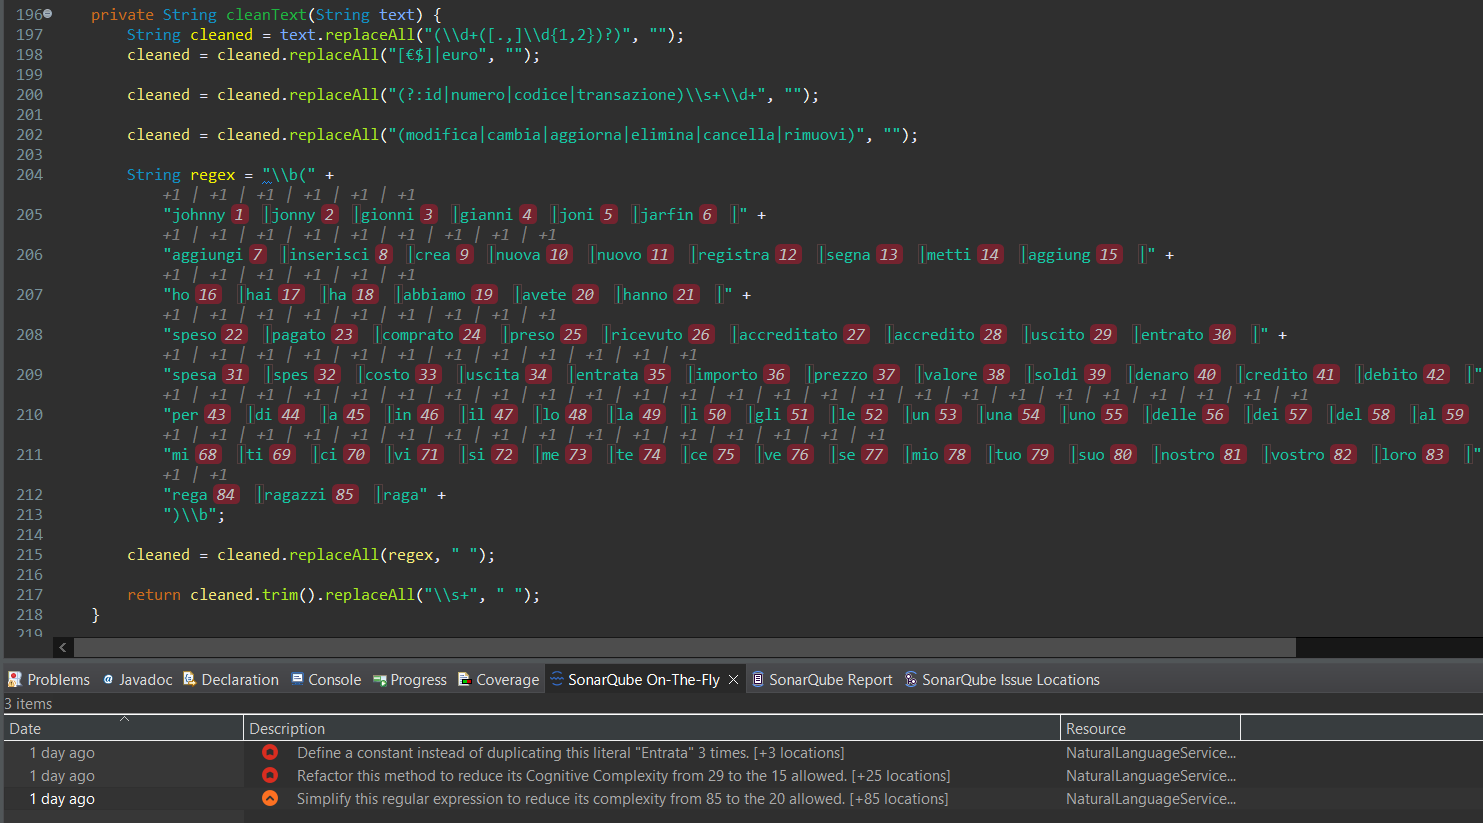
\includegraphics[width=0.75\textwidth]{../Iterazione_3/images/regex.png}
    \caption{segnalazione complessità regex}
    \label{fig:sonar_regex}
\end{figure}

\subsection{Testing di Integrazione e Resilienza}

Il \texttt{CommandController} funge da gateway applicativo per le richieste vocali. I test di integrazione hanno coperto scenari complessi e verificato la capacità del sistema di gestire i fallimenti dei microservizi a valle (\textit{Fault Tolerance}).

\subsubsection{Scenari Avanzati (NLU)}
Il seguente test verifica la corretta interpretazione di comandi basati sulla descrizione (es. "Cancella l'ultima pizza"), assicurando che il controller orchestratore invochi correttamente il servizio NLU e filtri i risultati.

\bigskip

\begin{lstlisting}[language=Java]
@Test
void process_Delete_ByDescription() throws Exception {
    // Scenario: Input vocale "Elimina pizza" -> Il sistema deve trovare l'ID corretto
    parsedTx.setDescription("pizza");
    when(nluService.parse(anyString())).thenReturn(parsedTx);
    
    // Il mock restituisce una lista, il controller filtra e ordina per data
    when(restTemplate.exchange(...)).thenReturn(ResponseEntity.ok(mockList));

    mockMvc.perform(post("/api/voice/process")...)
            .andExpect(jsonPath("$.message").value("Eliminato ID 20"));
}
\end{lstlisting}

\newpage

\subsubsection{Resilienza e Graceful Degradation}
In un'architettura a microservizi, il fallimento di un nodo backend è un evento atteso. È stata quindi implementata una strategia di \textit{Graceful Degradation}: se un servizio (es. Analytics) è irraggiungibile, l'interfaccia deve rimanere navigabile.

Il test seguente simula un rifiuto della connessione (\texttt{Connection refused}) e verifica che la Dashboard venga comunque servita con un messaggio di errore gestito, evitando il crash dell'applicazione (White Screen of Death).

\begin{lstlisting}[language=Java]
@Test
@DisplayName("HOME: Gestione errore Backend Down - Graceful Degradation")
void home_ShouldHandleBackendError() throws Exception {
    // 1. Simuliamo il fallimento del microservizio esterno
    when(restTemplate.getForObject(anyString(), eq(FinancialReport.class)))
        .thenThrow(new RestClientException("Connection refused"));

    // 2. Verifichiamo che la pagina venga comunque servita (HTTP 200)
    mockMvc.perform(get("/"))
        .andExpect(status().isOk())
        .andExpect(view().name("index"))
        .andExpect(model().attributeExists("error")); // Verifica presenza messaggio errore
}
\end{lstlisting}

\newpage

\subsection{Validazione Architetturale: API Gateway}

Per verificare il corretto instradamento delle richieste attraverso l'\texttt{api-gateway}, sono stati eseguiti test manuali con Postman puntando esclusivamente alla porta pubblica \texttt{8080}.

\begin{figure}[H]
    \centering
    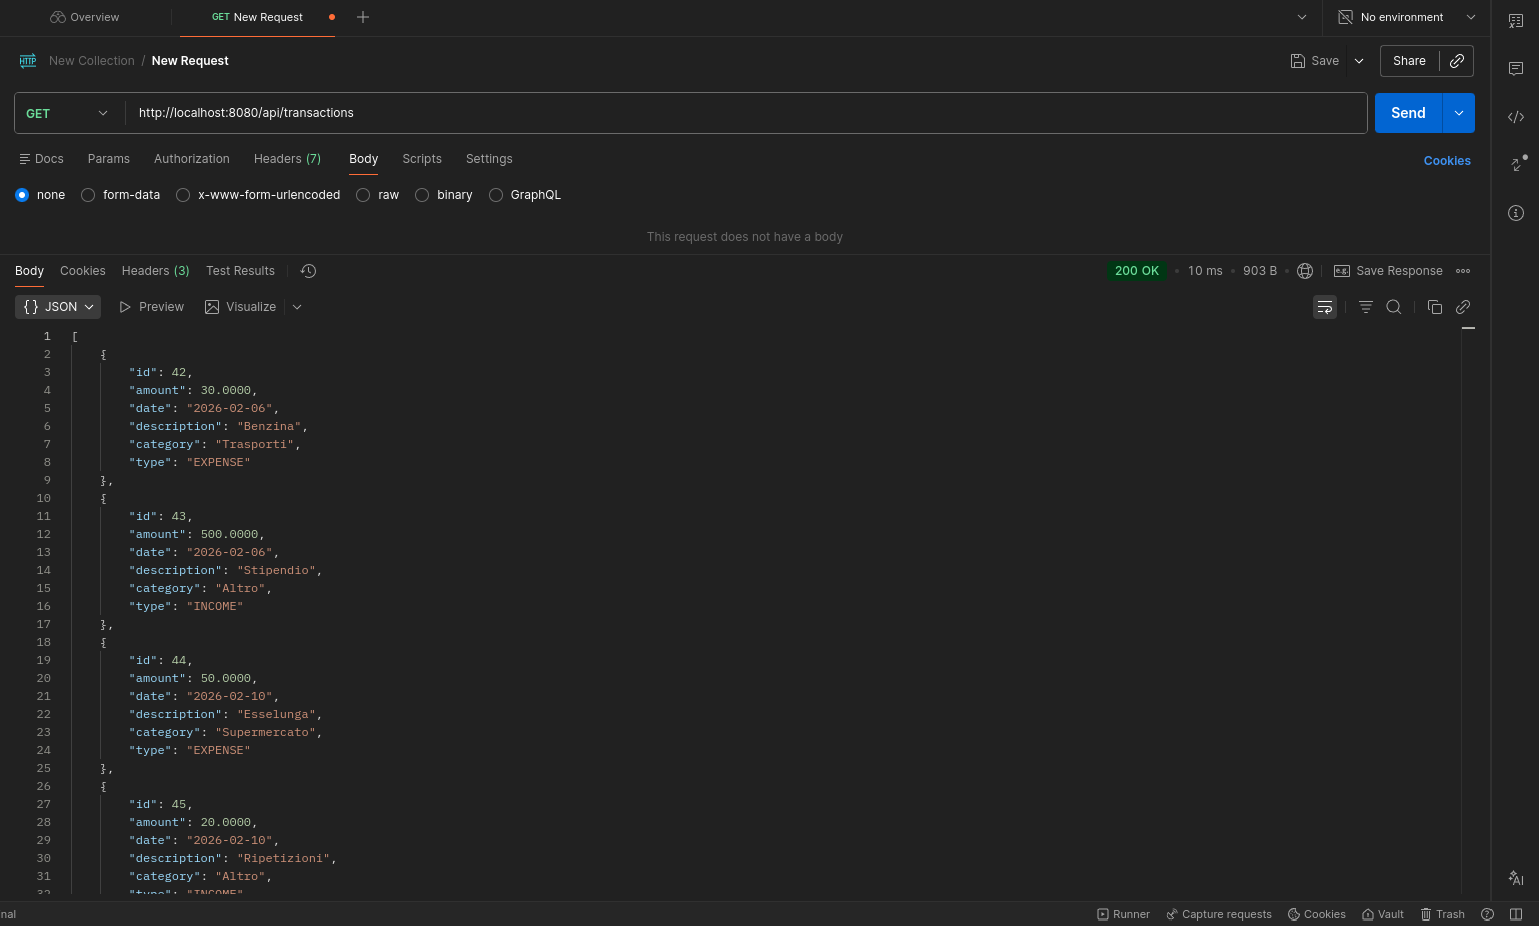
\includegraphics[width=0.85\textwidth]{../Iterazione_3/images/Routing_Accounting.png}
    \caption{Routing corretto verso Accounting Service via Gateway (Porta 8080)}
    \label{fig:routing_accounting}
\end{figure}

Le Figure \ref{fig:routing_accounting} e \ref{fig:routing_analytics} confermano che il Gateway agisce correttamente da \textit{Reverse Proxy}, mascherando la topologia interna dei microservizi (Accounting su 8081, Analytics su 8082) e offrendo un unico punto di accesso.

\begin{figure}[H]
    \centering
    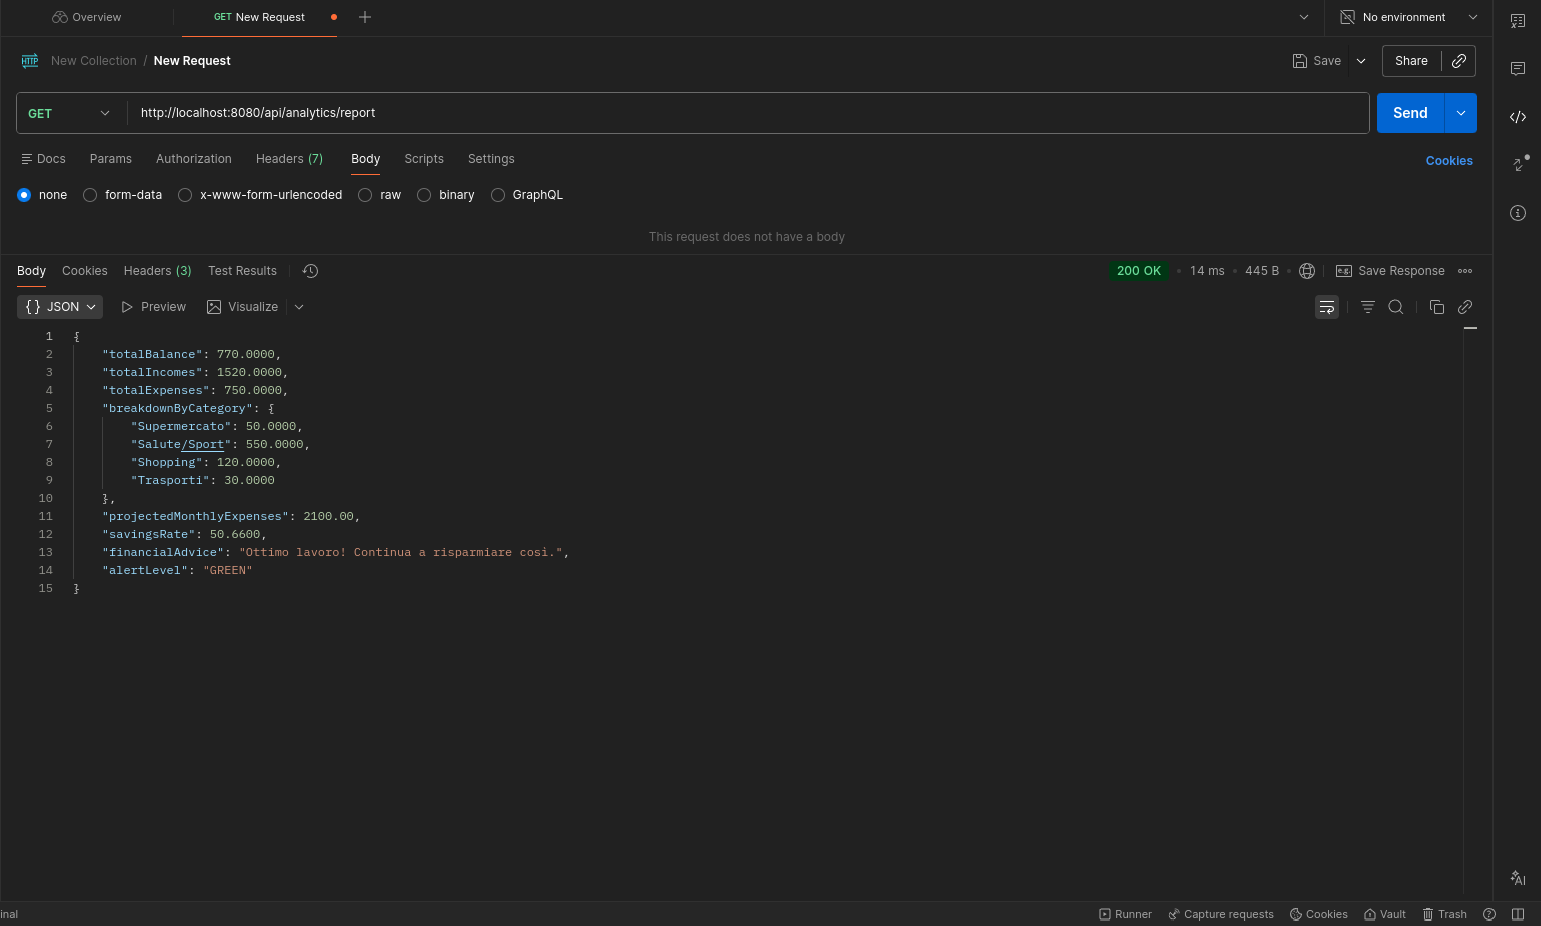
\includegraphics[width=0.85\textwidth]{../Iterazione_3/images/Routing_Analytics.png}
    \caption{Routing corretto verso Analytics Service via Gateway}
    \label{fig:routing_analytics}
\end{figure}

\subsection{Validazione Funzionale: Flusso Utente (UX)}

La validazione finale ha coinvolto l'interfaccia utente (Web UI), verificando l'esperienza d'uso complessiva.

\subsubsection{Inserimento Vocale}
Il test "sul campo" ha confermato l'efficacia del flusso \textit{Voice-to-Action}. Pronunciando \textit{"Ho speso 550 come abbonamento in palestra"}, il sistema ha trascritto l'audio localmente, interpretato l'intento tramite NLU e categorizzato la spesa, aggiornando la UI in tempo reale.

\begin{figure}[H]
    \centering
    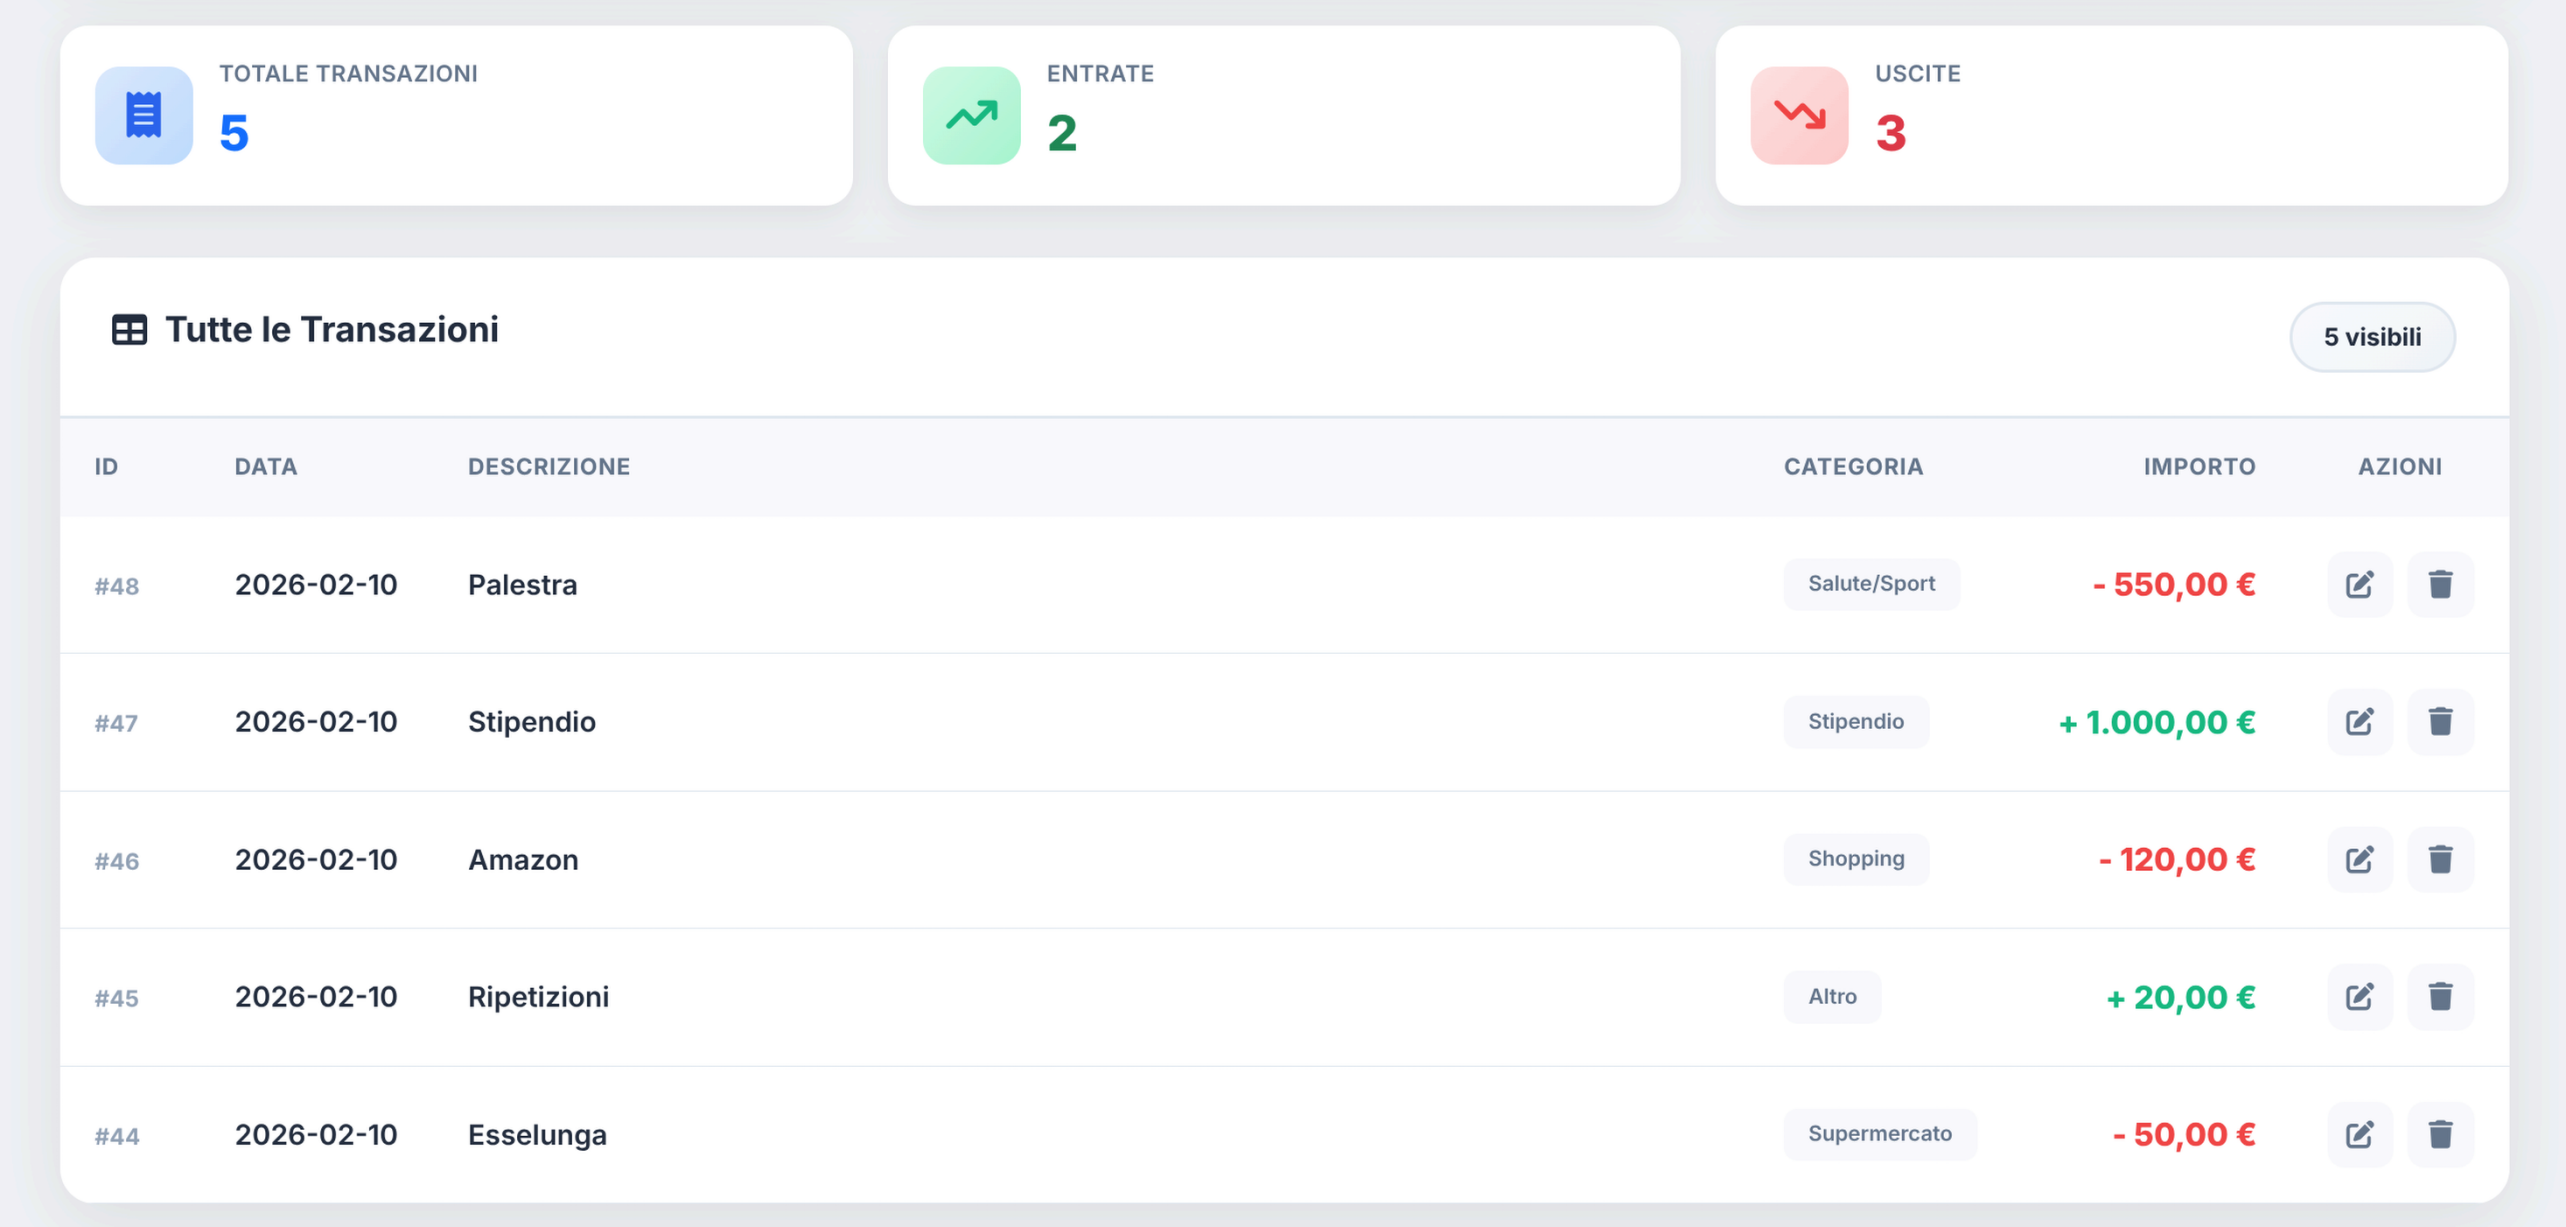
\includegraphics[width=1\textwidth]{../Iterazione_3/images/Inserimento_Vocale.png}
    \caption{Feedback visivo immediato dopo un comando vocale}
    \label{fig:inserimento_vocale}
\end{figure}

\newpage

\subsubsection{Gestione Errori UI}
In linea con i test di resilienza backend, è stato verificato il comportamento visivo in caso di guasto. Spegnendo il Gateway, la Web UI ha mostrato un alert chiaro all'utente (Figura \ref{fig:errore_gestito}), confermando il successo della strategia di \textit{Graceful Degradation}.

\begin{figure}[H]
    \centering
    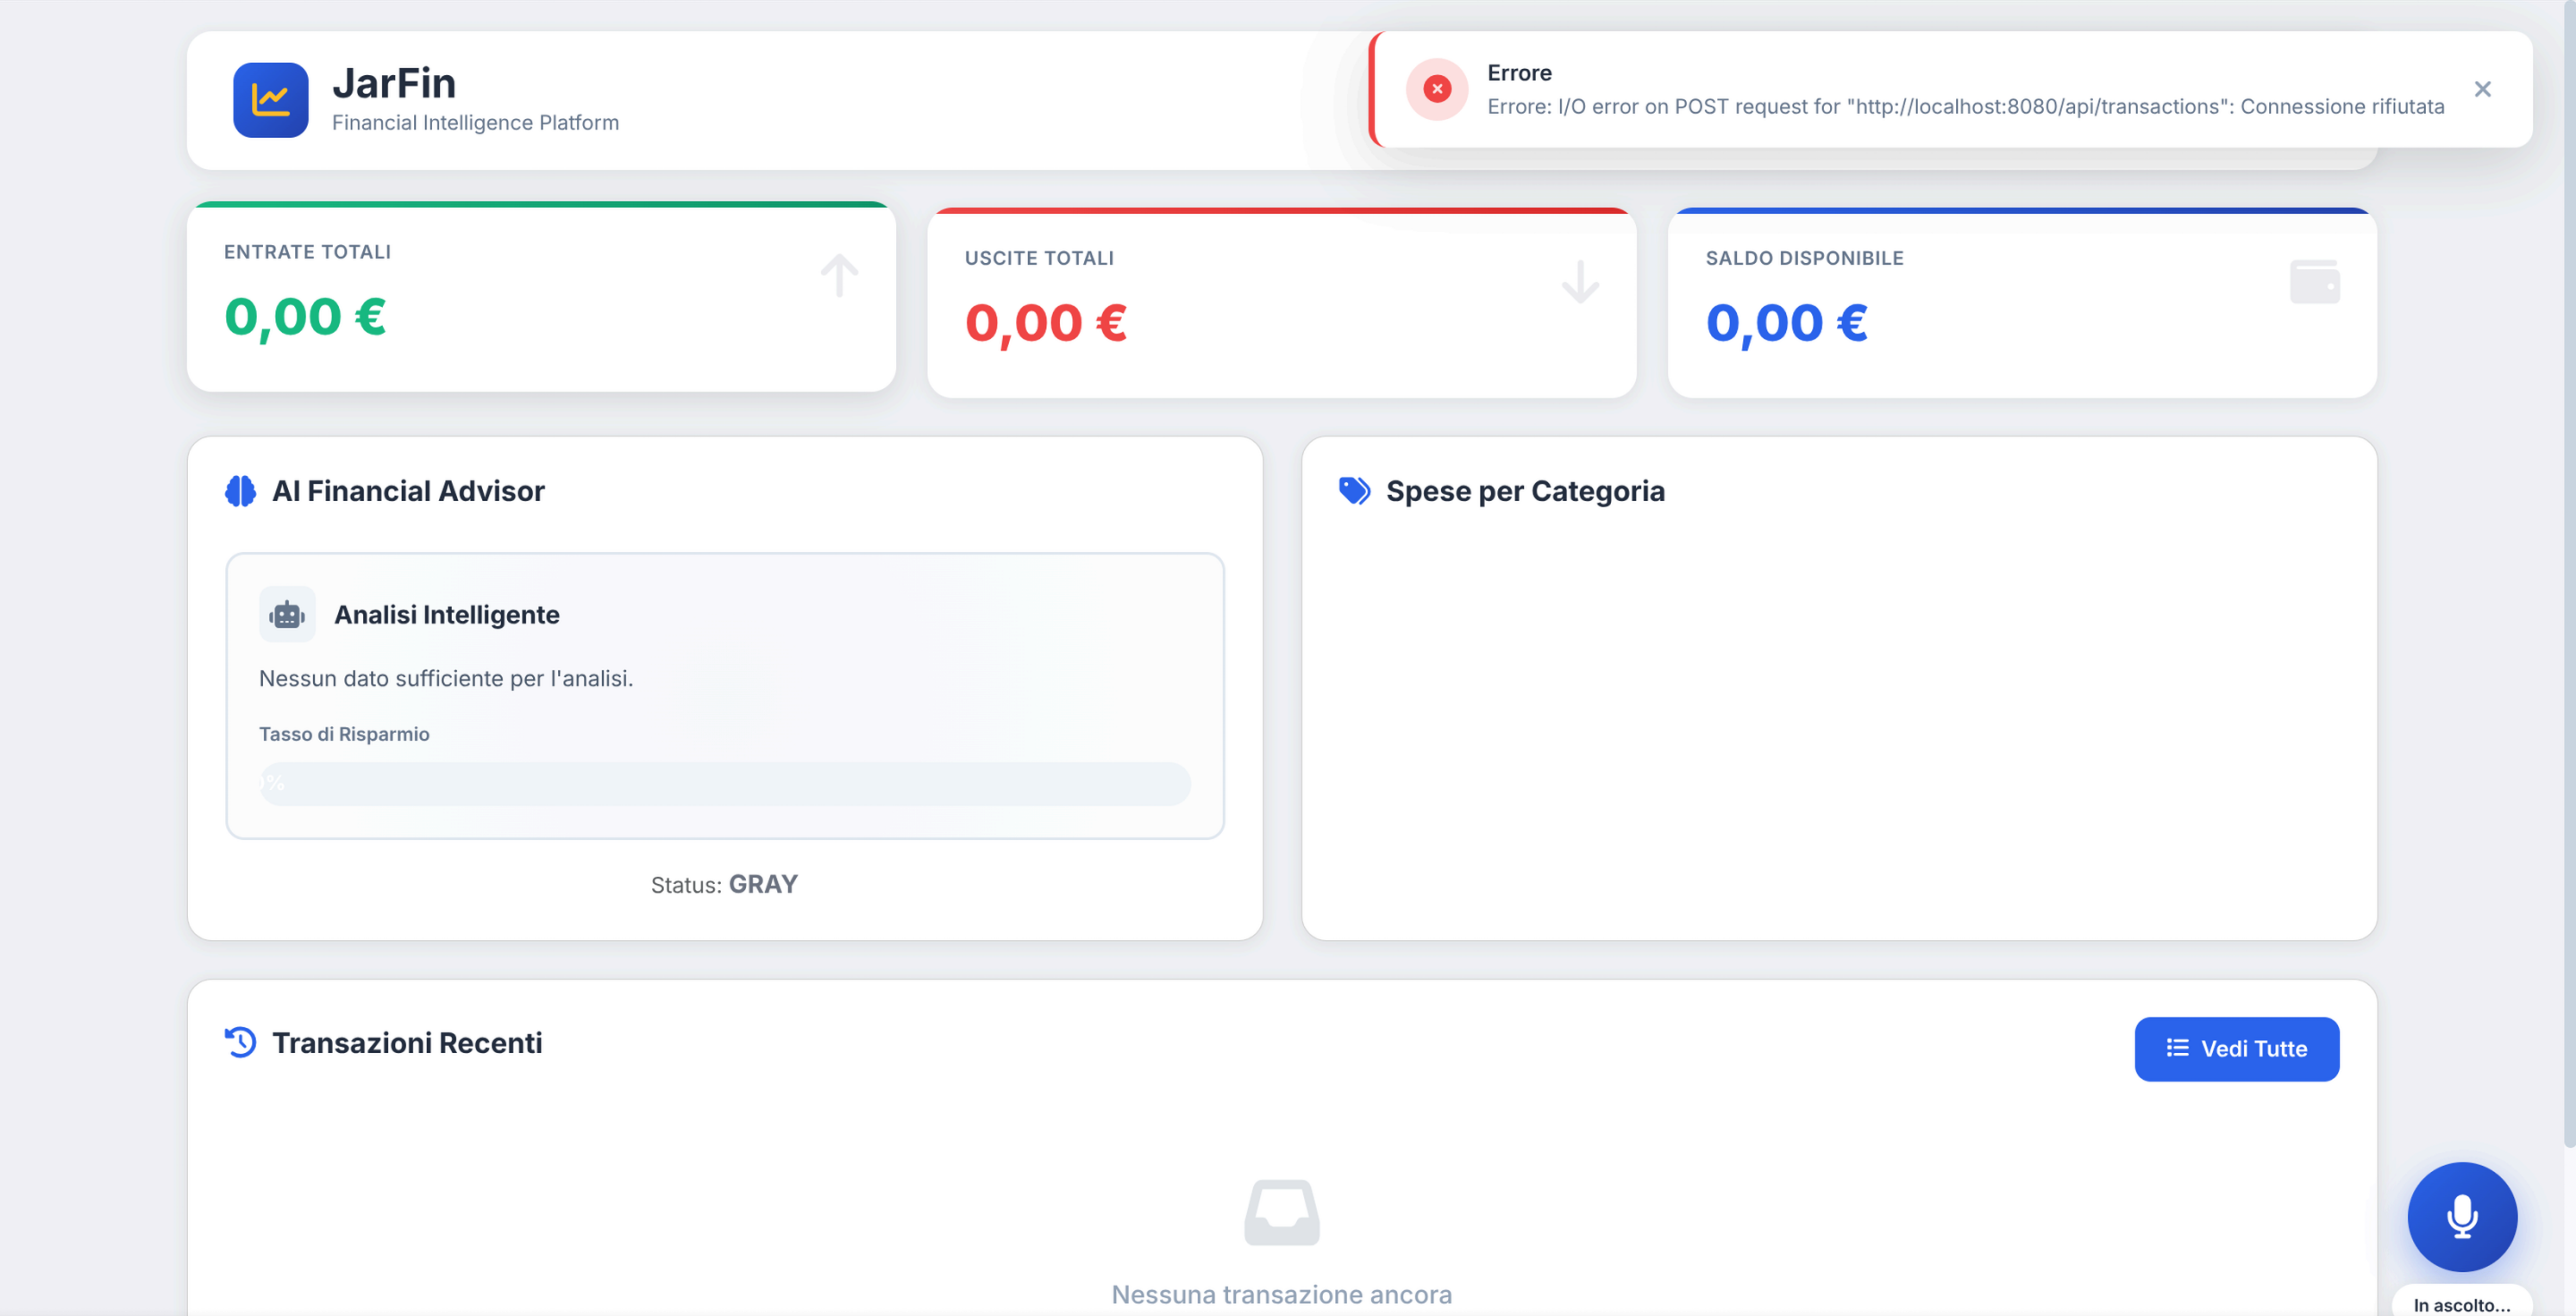
\includegraphics[width=0.95\textwidth]{../Iterazione_3/images/Errore_Gestito.png}
    \caption{UI Error Handling: Feedback visivo in caso di disservizio}
    \label{fig:errore_gestito}
\end{figure}

Inoltre, il sistema implementa un controllo di compatibilità browser (Feature Detection), avvisando l'utente se le Web Speech API non sono supportate (es. su Firefox).

\begin{figure}[H]
    \centering
    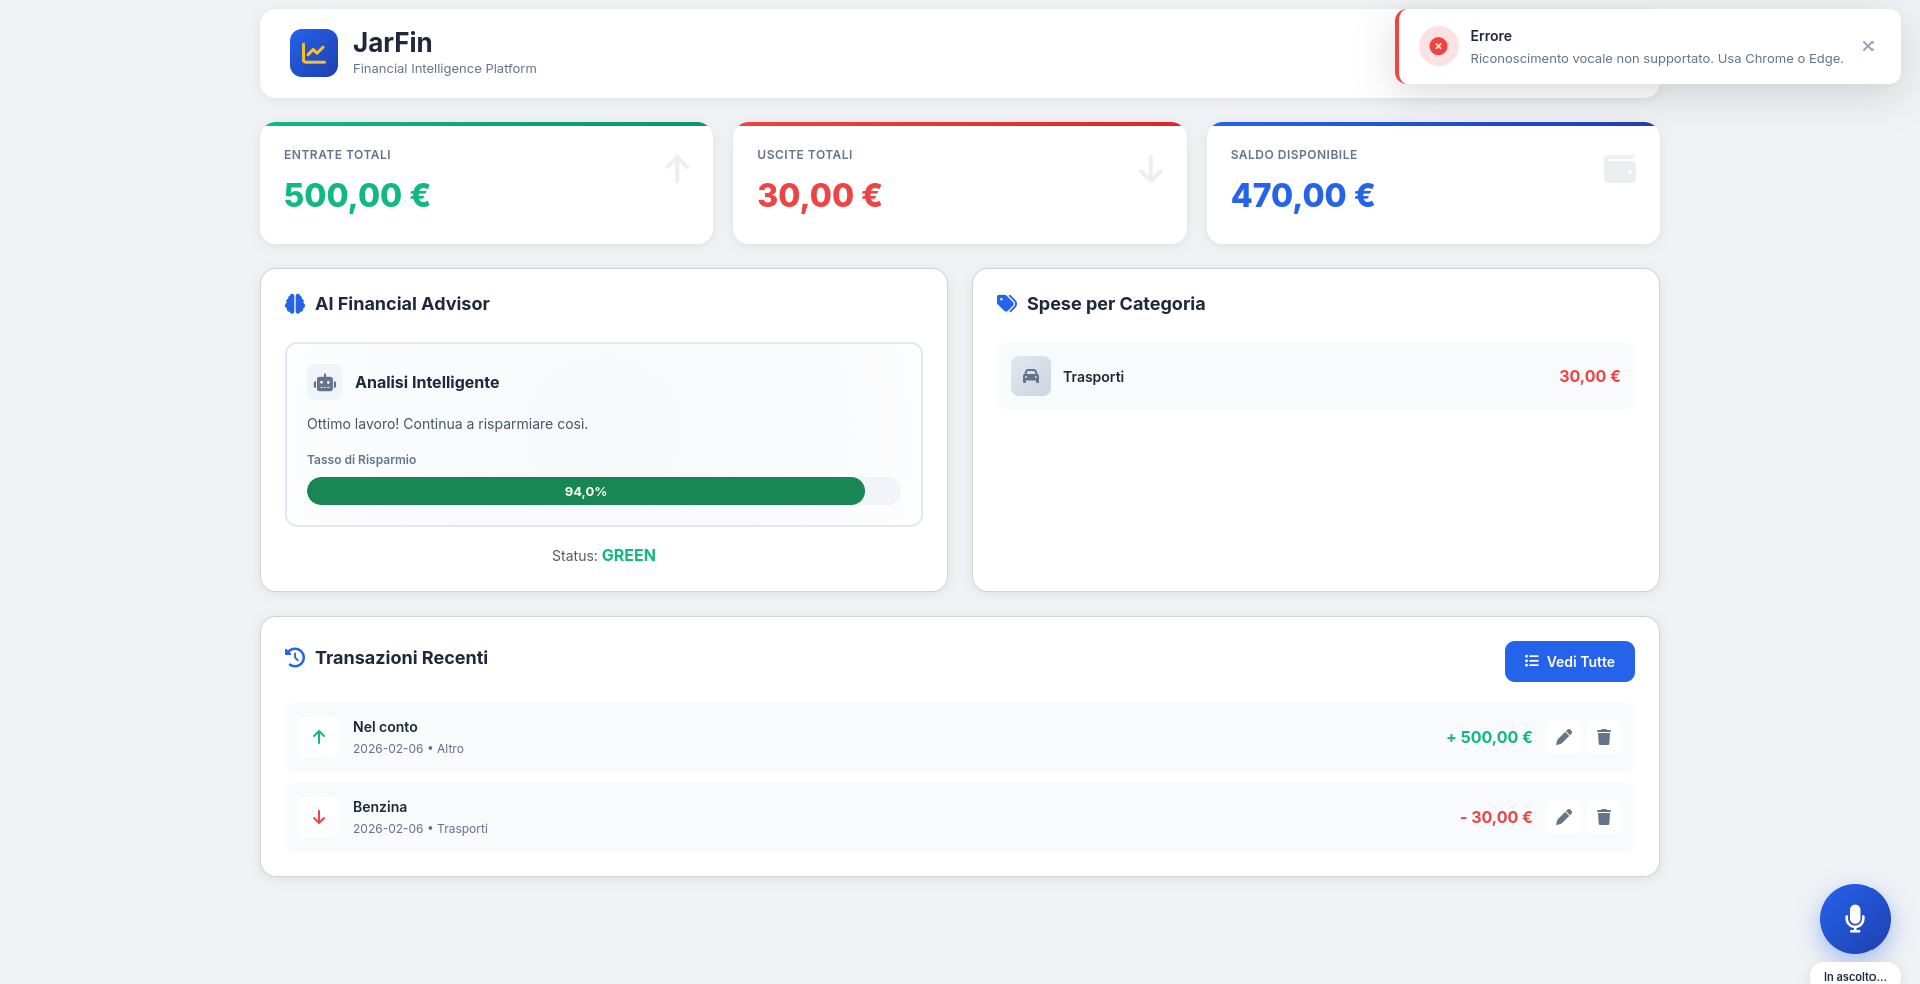
\includegraphics[width=0.95\textwidth]{../Iterazione_3/images/Firefox_error.png}
    \caption{Feature Detection: Avviso di incompatibilità browser}
    \label{fig:firefox_error}
\end{figure}

\subsubsection{Operazioni CRUD}
Infine, sono state validate le operazioni standard di modifica e cancellazione (Figure \ref{fig:modifica_transazione} e \ref{fig:cancellazione_transazione}) e il sistema di filtraggio, essenziali per la gestione quotidiana dei dati.

\begin{figure}[H]
    \centering
    \begin{minipage}{0.49\textwidth}
        \centering
        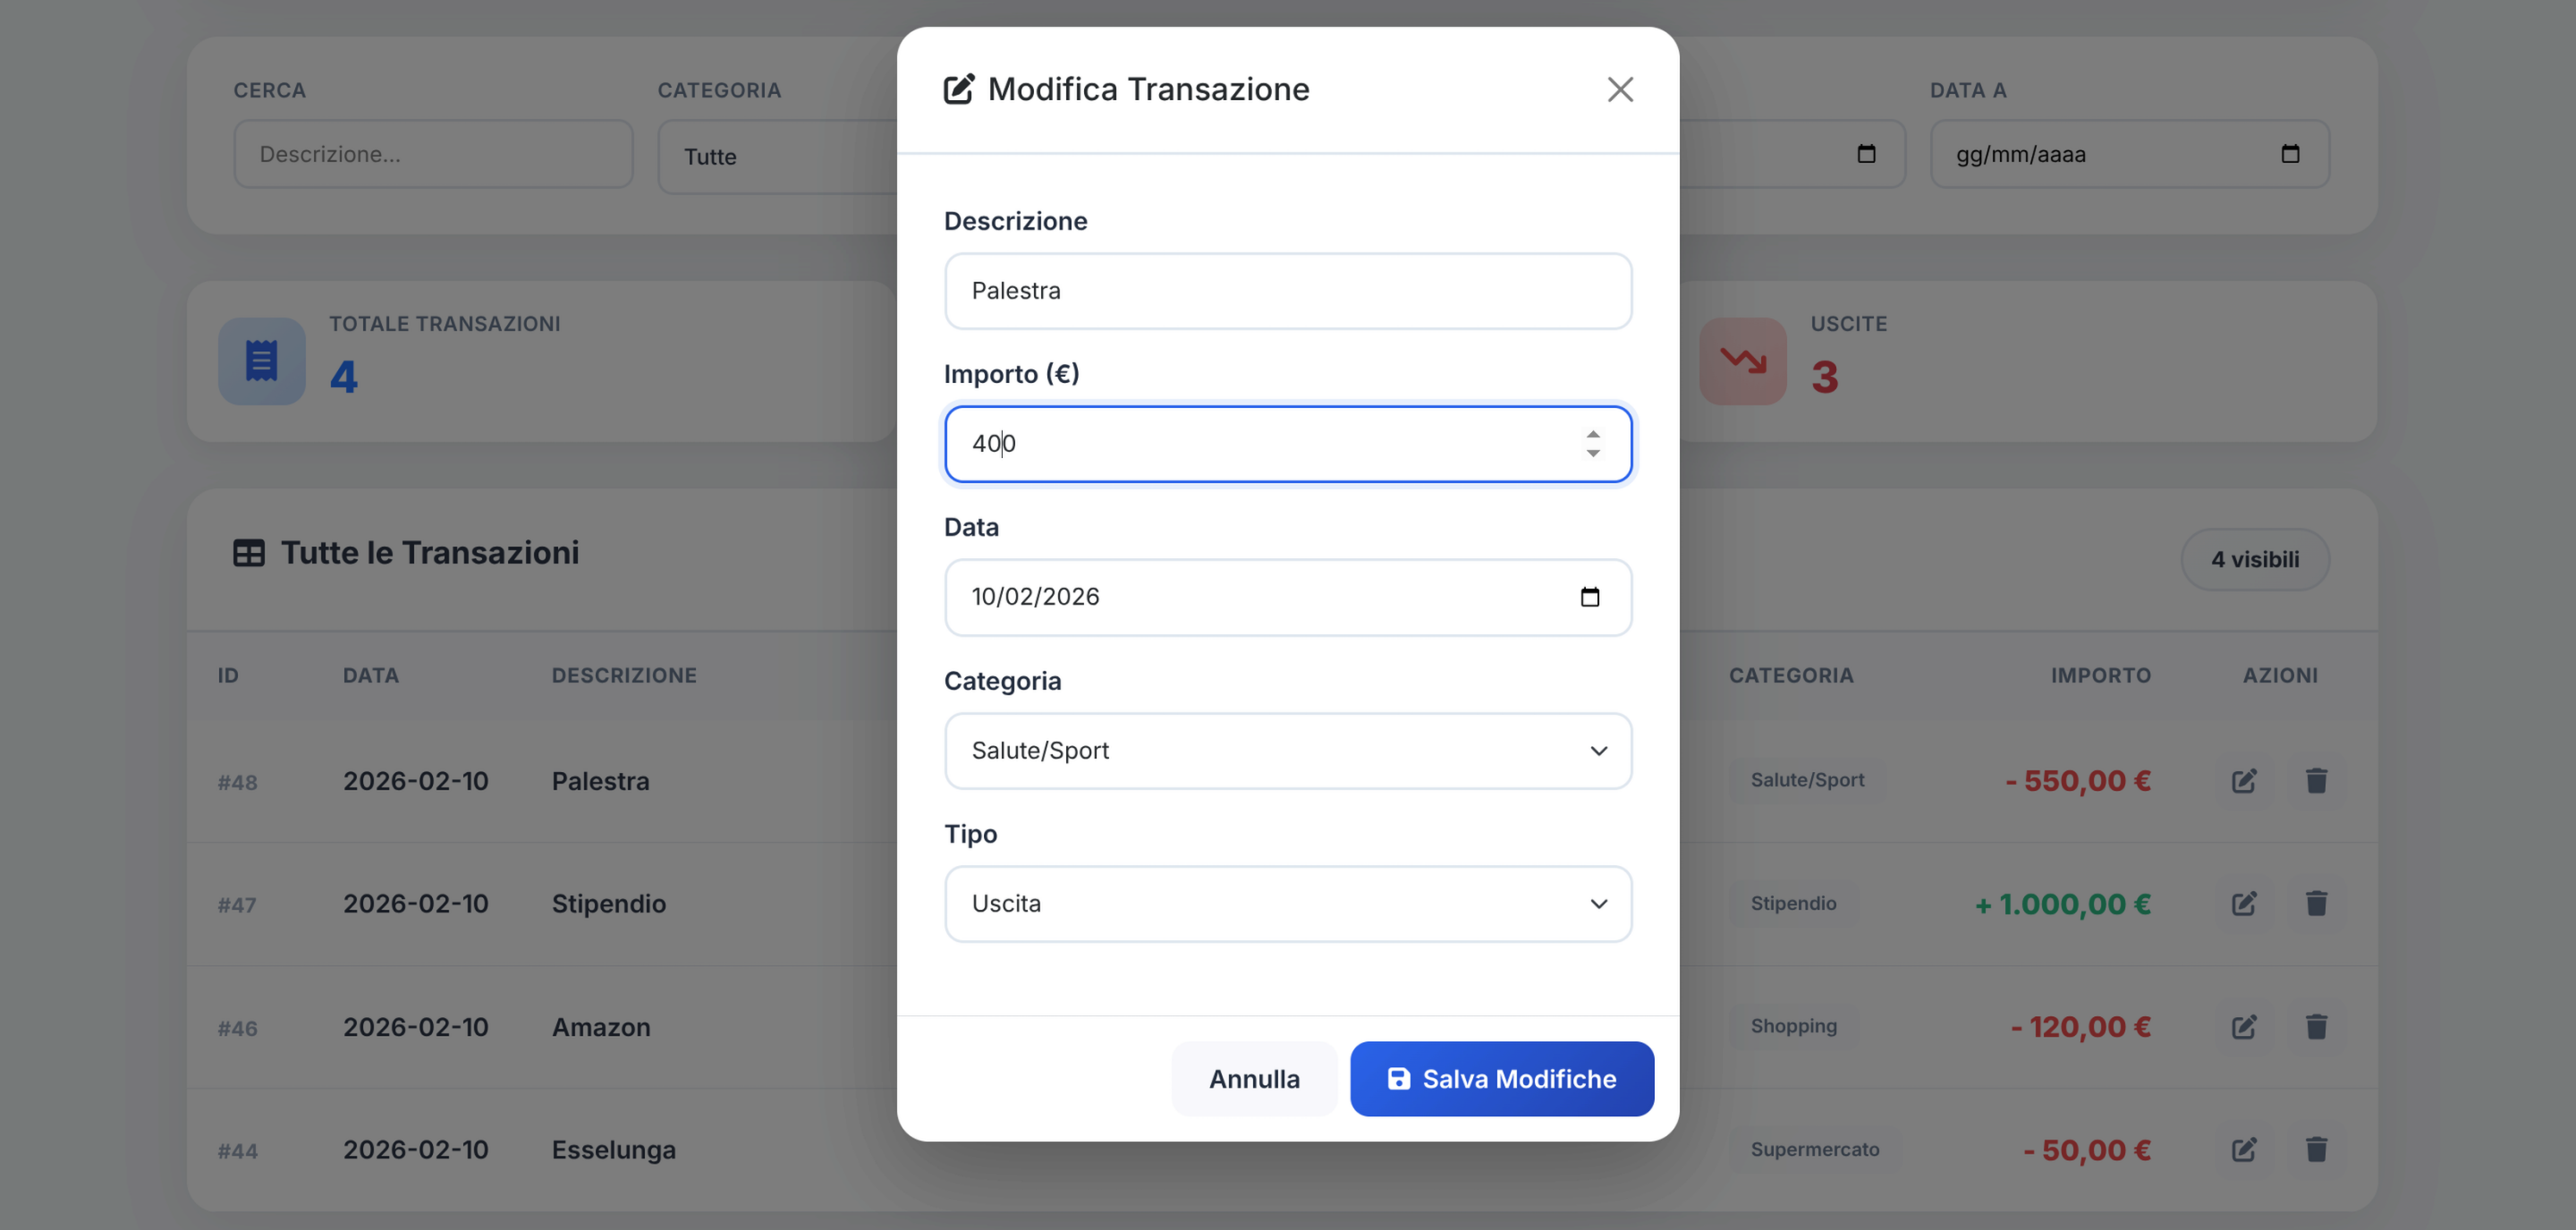
\includegraphics[width=\textwidth]{../Iterazione_3/images/Modifica_Transazione.png}
        \caption{Modifica Transazione}
        \label{fig:modifica_transazione}
    \end{minipage}
    \hfill
    \begin{minipage}{0.49\textwidth}
        \centering
        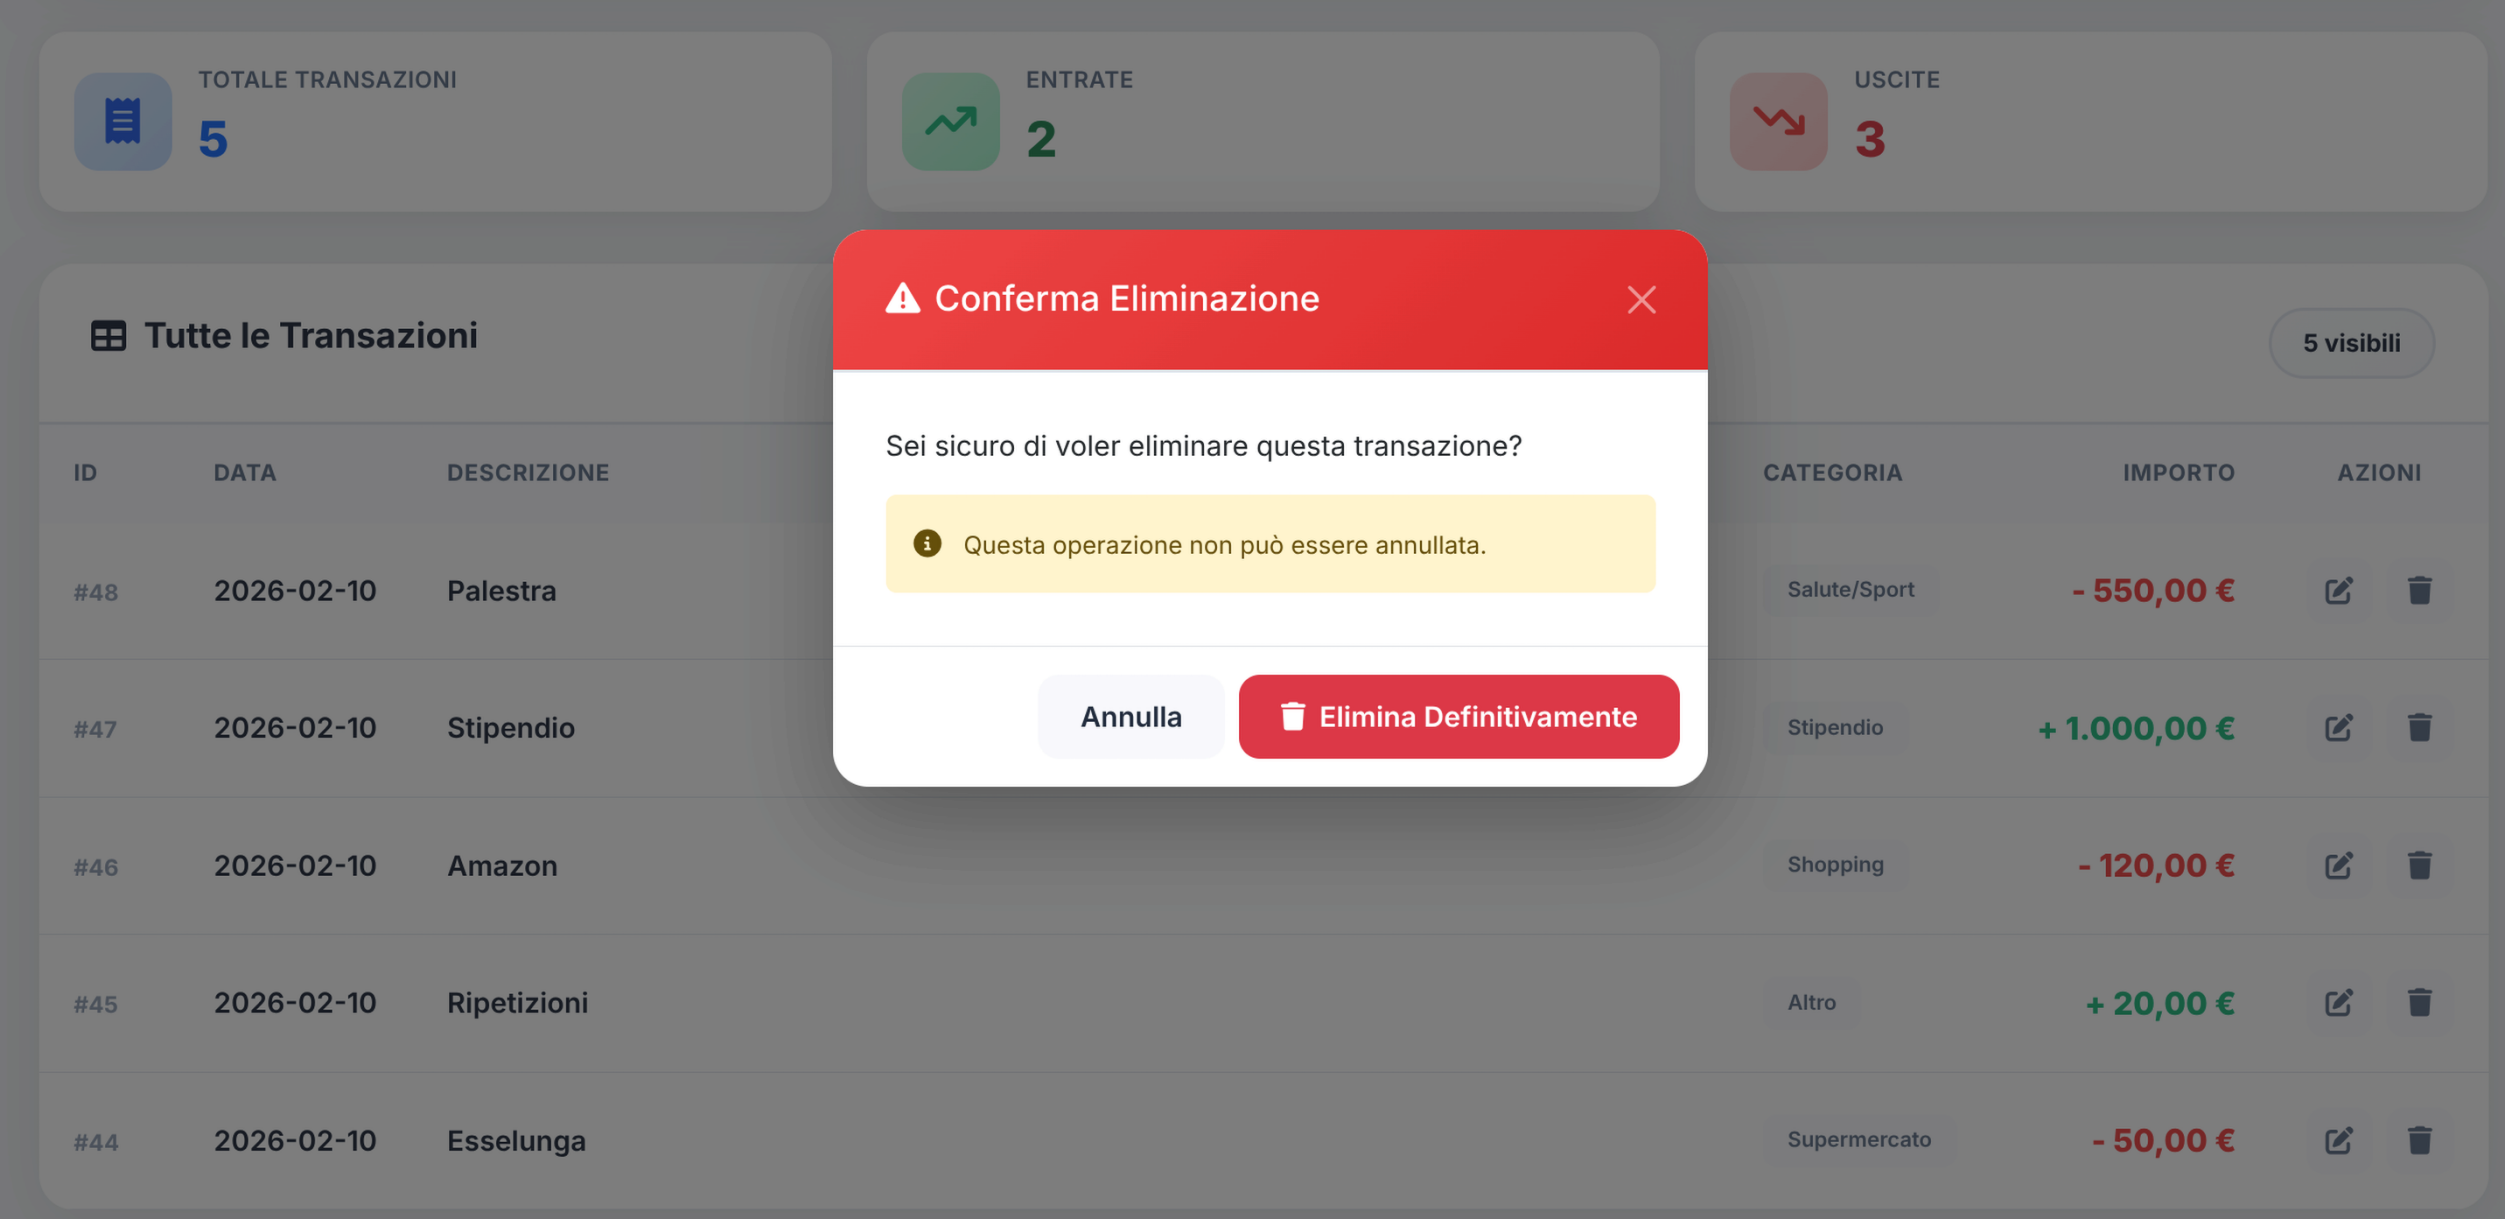
\includegraphics[width=\textwidth]{../Iterazione_3/images/Cancellazione_Transazione.png}
        \caption{Cancellazione Transazione}
        \label{fig:cancellazione_transazione}
    \end{minipage}
\end{figure}

\begin{figure}[H]
    \centering
    \begin{minipage}{0.49\textwidth}
        \centering
        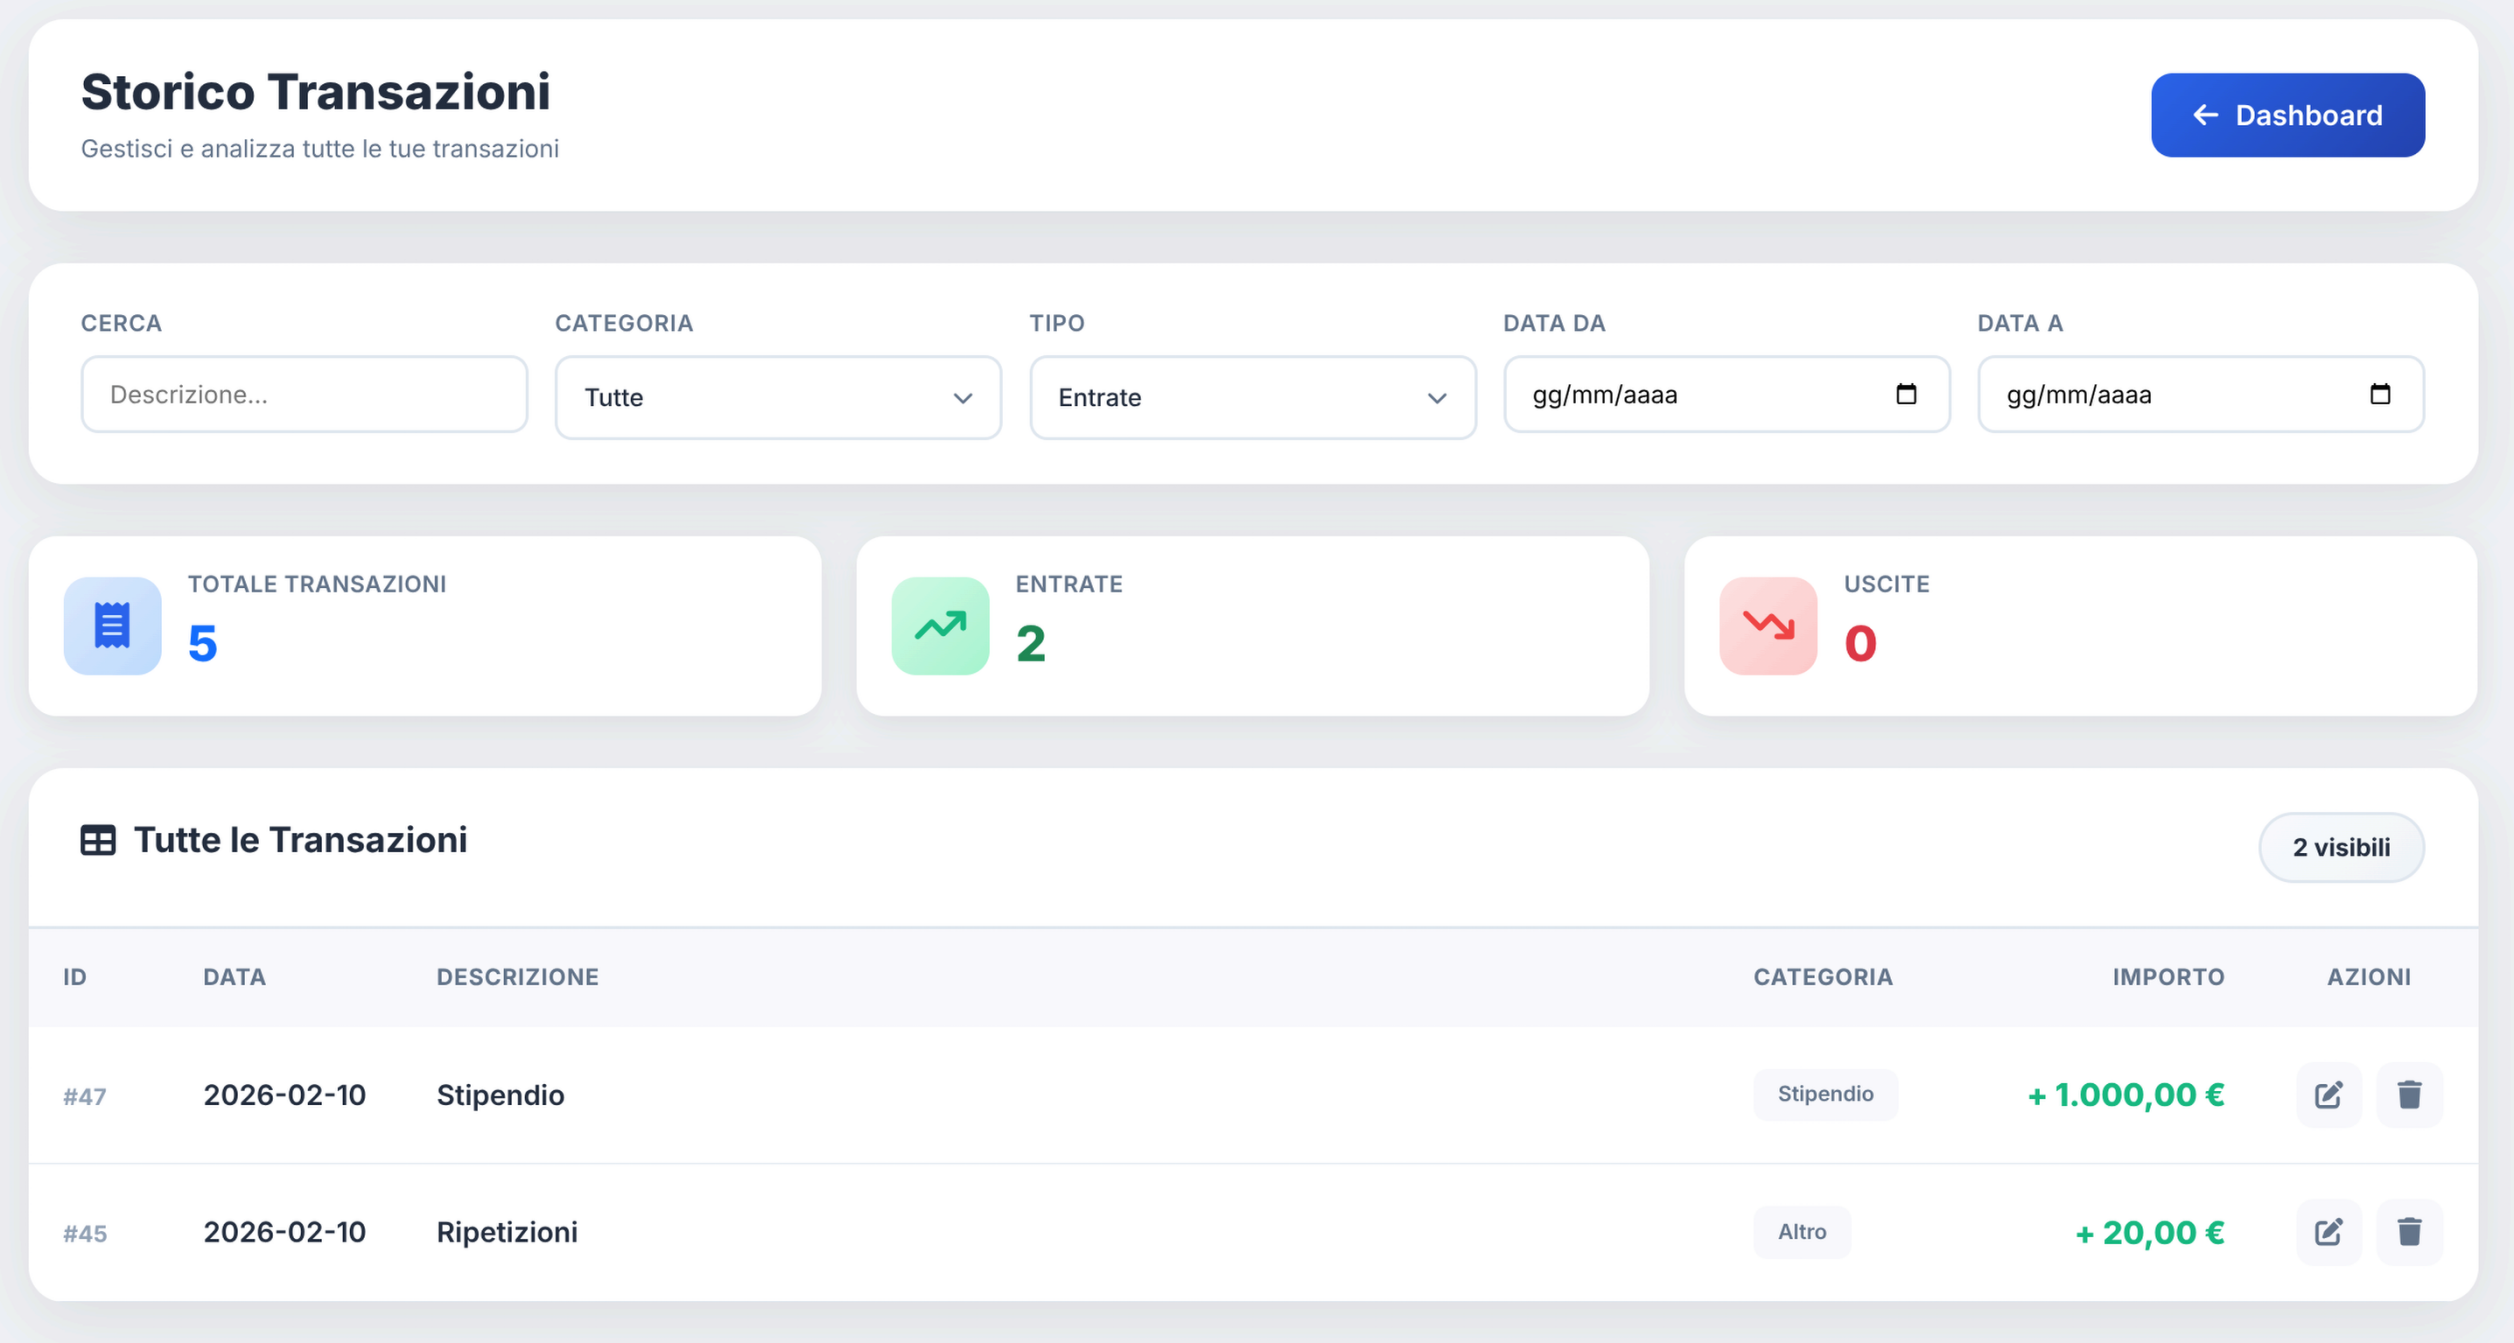
\includegraphics[width=\textwidth]{../Iterazione_3/images/Filtro_Entrate.png}
        \caption{Filtro Entrate}
        \label{fig:filtro_entrate}
    \end{minipage}
    \hfill
    \begin{minipage}{0.49\textwidth}
        \centering
        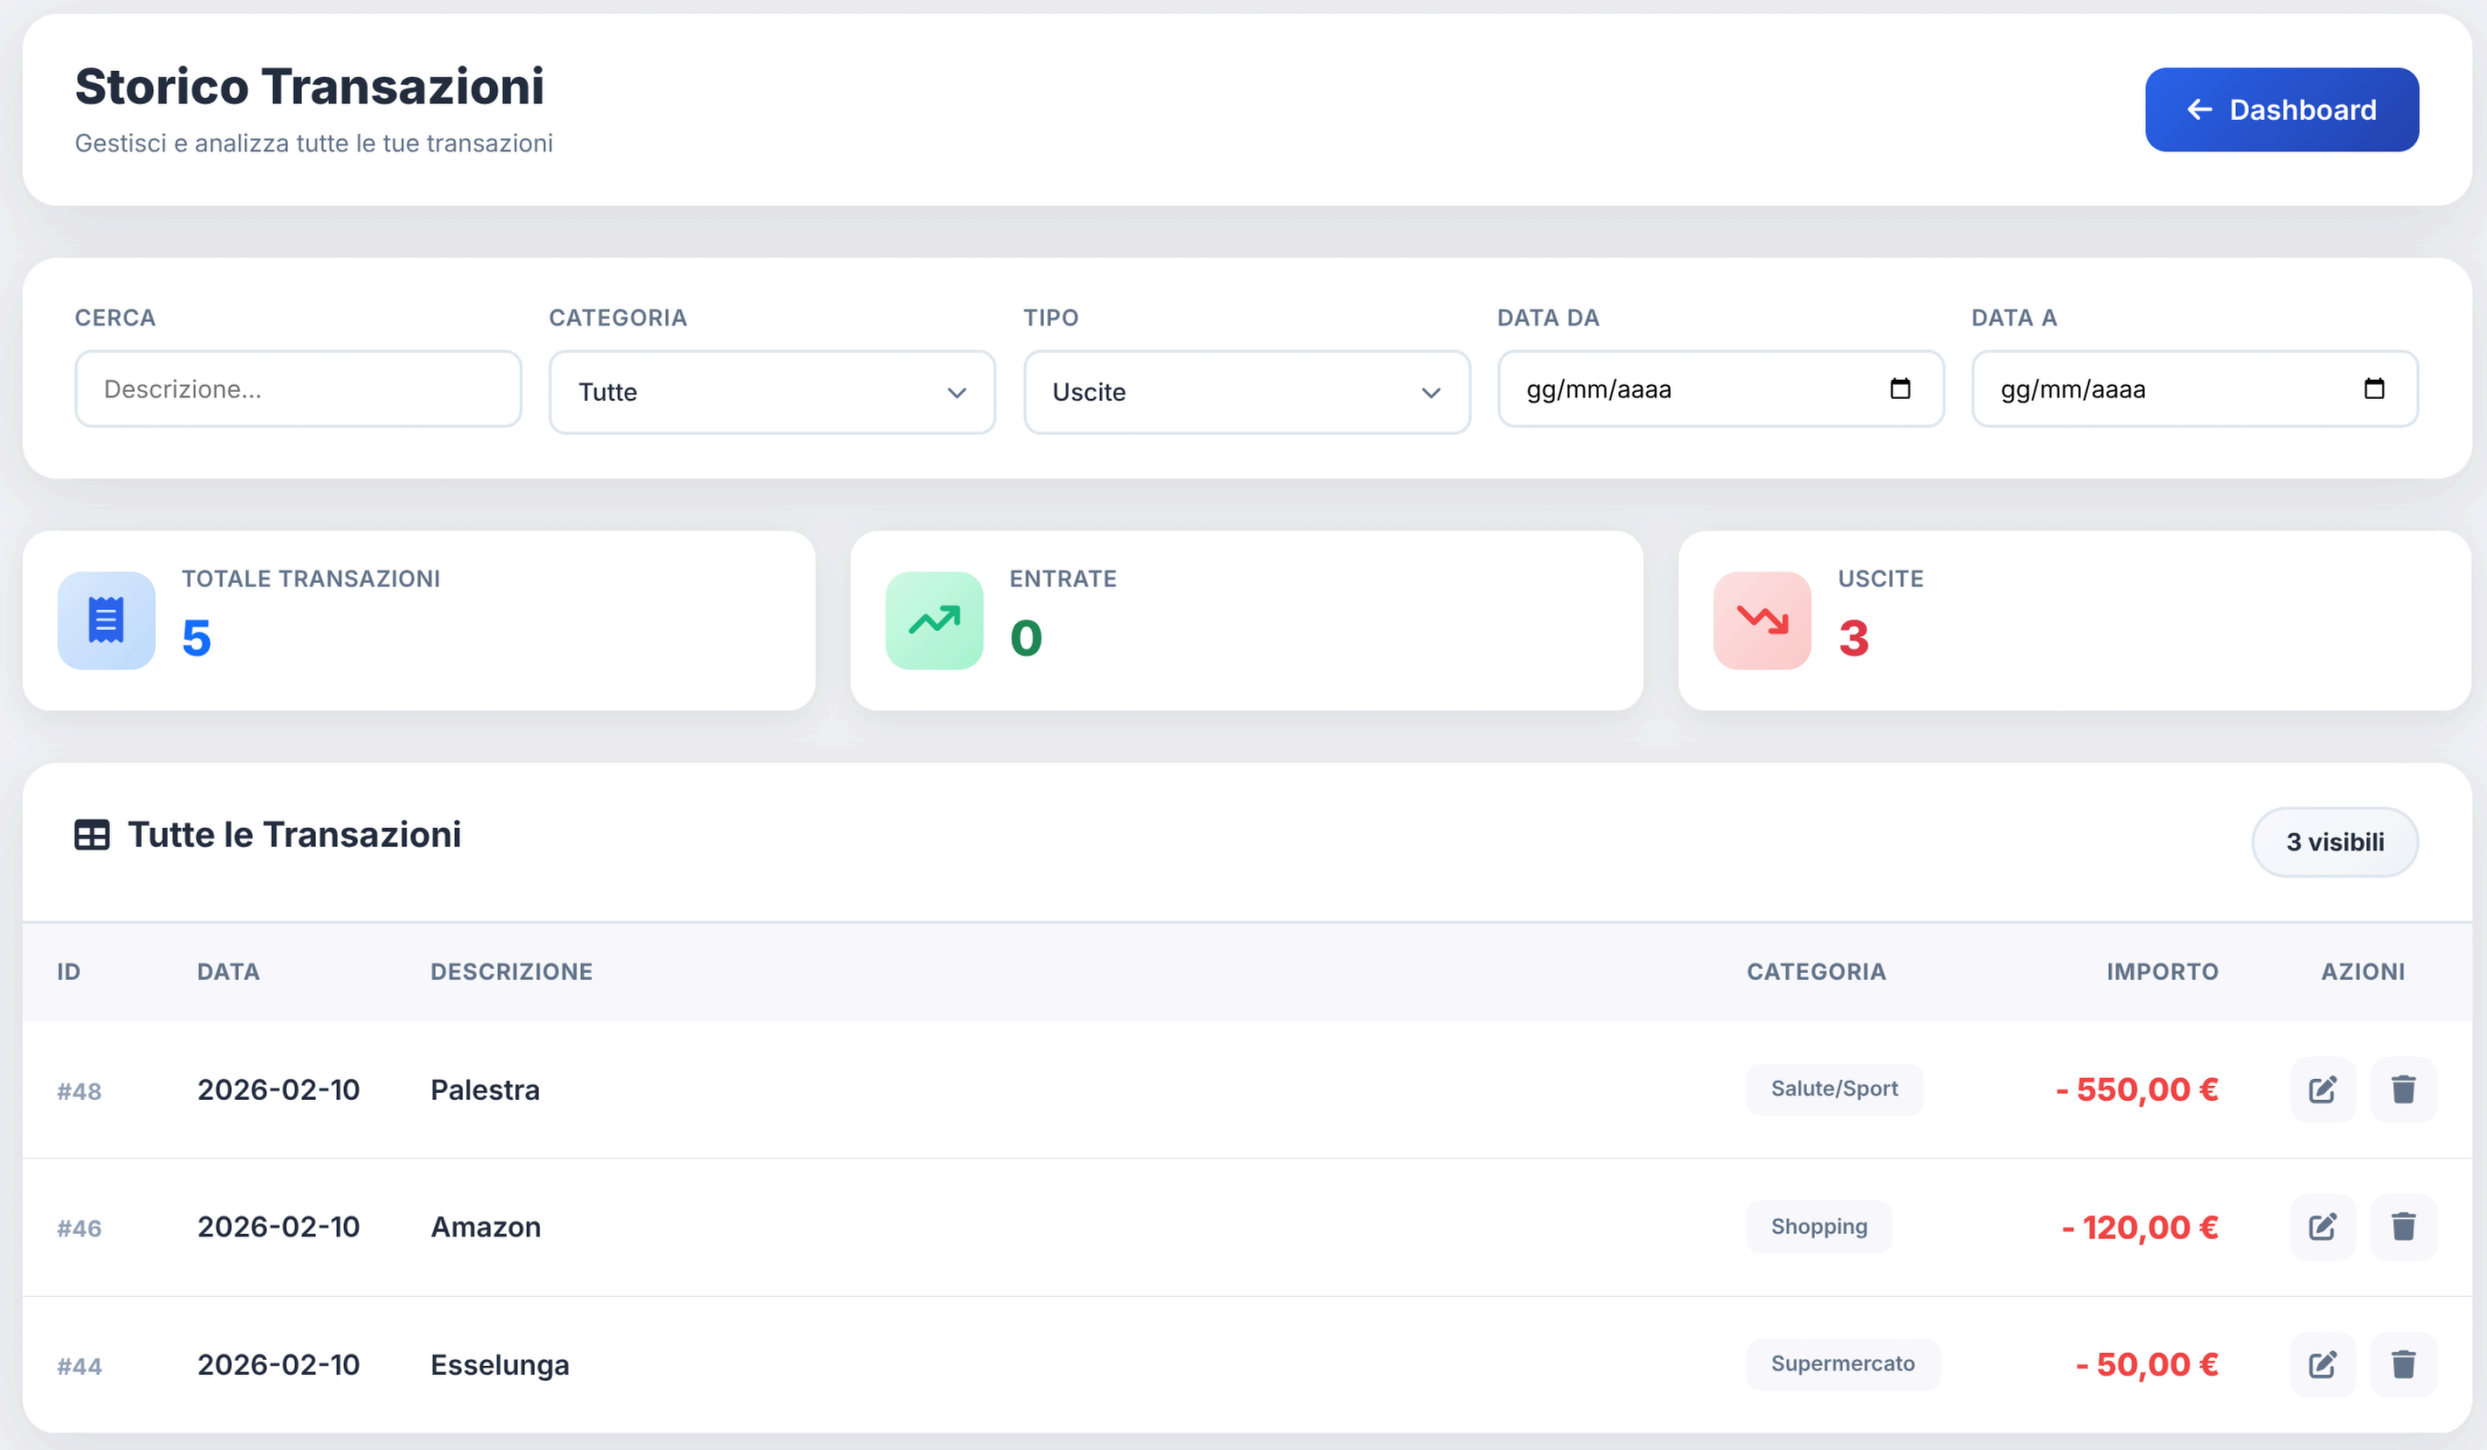
\includegraphics[width=\textwidth]{../Iterazione_3/images/Filtro_Uscite.png}
        \caption{Filtro Uscite}
        \label{fig:filtro_uscite}
    \end{minipage}
\end{figure}

\begin{figure}[H]
    \centering
    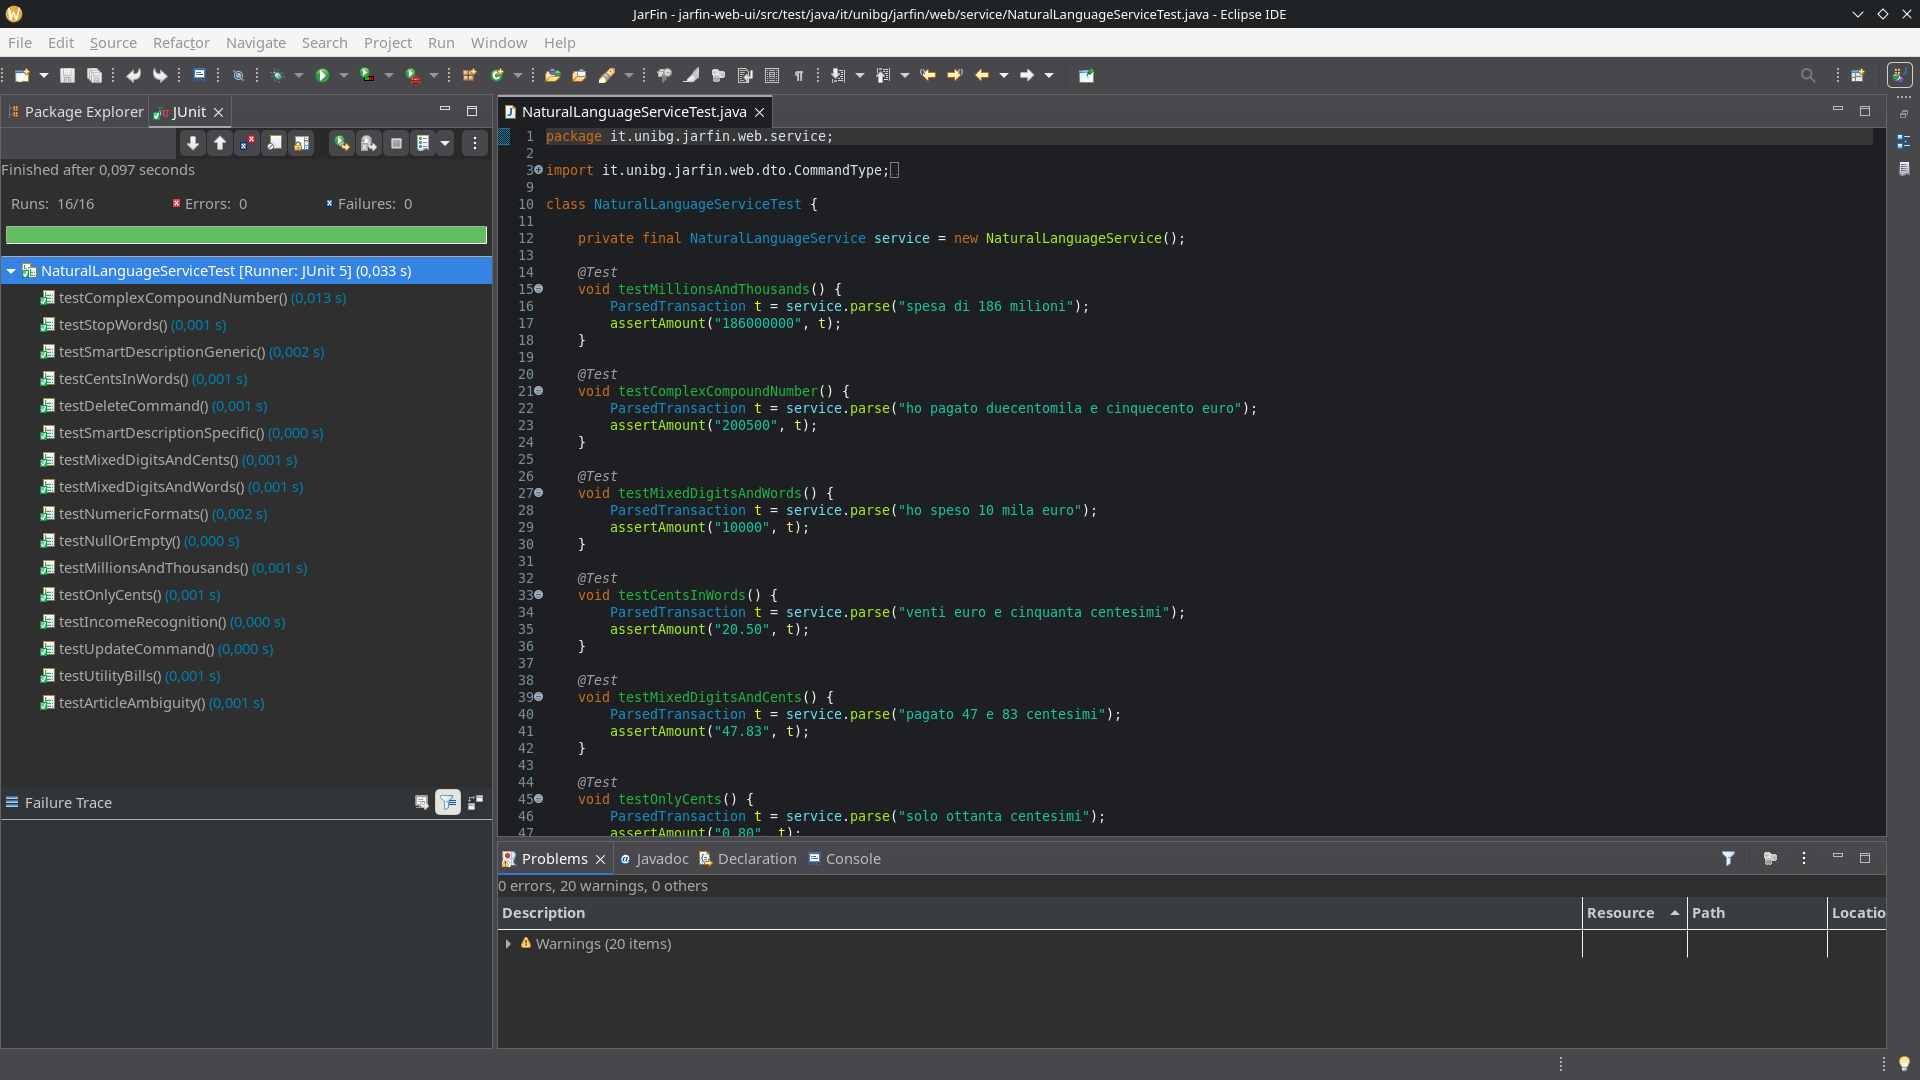
\includegraphics[width=1\textwidth]{../Iterazione_3/images/NaturalLanguageServiceTest.png}
    \caption{Routing corretto verso Analytics Service via Gateway}
    \label{fig:NaturalLanguageServiceTest}
\end{figure}

\newpage

\subsection{Metriche di Qualità Finali}

A conclusione dell'iterazione, le metriche di copertura confermano la robustezza del modulo Web UI, con una copertura quasi totale del Service Layer (NLU):

\begin{itemize}
    \item \textbf{Service Layer Coverage:} 98.5\%
    \item \textbf{Controller Layer Coverage:} 84.7\%
    \item \textbf{Web UI Package Coverage:} 95.8\%
\end{itemize}

L'analisi strutturale con \textbf{CodeMR} (Figure \ref{fig:codemr_web_quality} e \ref{fig:codemr_web_deps}) mostra un'architettura bilanciata, con una chiara separazione delle responsabilità tra i componenti di presentazione e logica.

\begin{figure}[H]
    \centering
    
\includegraphics[width=0.85\textwidth]{../Iterazione_3/images/quality-attributes.png}
    \caption{Metriche di qualità architetturale per il modulo web-ui}
    \label{fig:codemr_web_quality}
\end{figure}

\begin{figure}[H]
    \centering
    
\includegraphics[width=0.8\textwidth]{../Iterazione_3/images/dependencies.png}
    \caption{Grafo delle dipendenze del modulo web-ui}
    \label{fig:codemr_web_deps}
\end{figure}

\section{Conclusione Iterazione 3}

L'Iterazione 3 ha rappresentato il punto di svolta per il progetto \textit{JarFin}, trasformando un insieme di microservizi backend in una \textbf{piattaforma applicativa completa}.

I risultati raggiunti coprono l'intero stack:
\begin{itemize}
    \item \textbf{Infrastruttura}: L'API Gateway ha unificato i punti di accesso, garantendo sicurezza e disaccoppiamento.
    \item \textbf{Frontend}: La Web UI ha offerto una dashboard interattiva e un'esperienza moderna ("Voice First").
    \item \textbf{Intelligenza}: Il motore NLU deterministico ha dimostrato che è possibile interpretare il linguaggio naturale con complessità $O(n)$, offrendo un'alternativa robusta e privata ai modelli Cloud.
\end{itemize}

Il sistema è ora pienamente operativo in tutte le sue componenti: interfaccia, logica di business e persistenza.